\documentclass[12pt]{article}
% Load packages
\usepackage{url}  % Formatting web addresses  
\usepackage{ifthen}  % Conditional 
\usepackage{multicol}   %Columns
\usepackage[utf8]{inputenc} %unicode support
\usepackage{amsmath}
\usepackage{amssymb}
\usepackage{epsfig}
\usepackage{epstopdf}
\usepackage{graphicx}
\usepackage[margin=0.1pt,font=footnotesize,labelfont=bf]{caption}
\usepackage{setspace}
%\usepackage{longtable}
\usepackage{colortbl}
%\usepackage{palatino,lettrine}
%\usepackage{times}
%\usepackage[applemac]{inputenc} %applemac support if unicode package fails
%\usepackage[latin1]{inputenc} %UNIX support if unicode package fails
\usepackage[wide]{sidecap}
%\usepackage[authoryear,round,comma,sort&compress]{natbib}
\usepackage[square,sort&compress,comma,numbers]{natbib}
%\usepackage[authoryear,round]{natbib}
\usepackage{supertabular}
\usepackage{simplemargins}
\usepackage{comment}
\usepackage{lineno}

\urlstyle{rm}

%\textwidth = 6.50 in
%\textheight = 9.5 in
%\oddsidemargin =  0.0 in
%\evensidemargin = 0.0 in
%\topmargin = -0.50 in
%\headheight = 0.0 in
%\headsep = 0.25 in
%\parskip = 0.15in
%\linespread{1.75}
\doublespace

%\usepackage{geometry}
\usepackage{fullpage}

%\bibliographystyle{plain}
\bibliographystyle{plos2009}

\makeatletter
\renewcommand\subsection{\@startsection
	{subsection}{2}{0mm}
	{-0.05in}
	{-0.5\baselineskip}
	{\normalfont\normalsize\bfseries}}
\renewcommand\subsubsection{\@startsection
	{subsubsection}{2}{0mm}
	{-0.05in}
	{-0.5\baselineskip}
	{\normalfont\normalsize\itshape}}
\renewcommand\section{\@startsection
	{subsection}{2}{0mm}
	{-0.2in}
	{0.05\baselineskip}
	{\normalfont\large\bfseries}}	
\renewcommand\paragraph{\@startsection
	{paragraph}{2}{0mm}
	{-0.05in}
	{-0.5\baselineskip}
	{\normalfont\normalsize\itshape}}
\makeatother

%Review style settings
%\newenvironment{bmcformat}{\begin{raggedright}\baselineskip20pt\sloppy\setboolean{publ}{false}}{\end{raggedright}\baselineskip20pt\sloppy}

%Publication style settings

% Single space'd bib -
\setlength\bibsep{0pt}

\renewcommand{\rmdefault}{phv}\renewcommand{\sfdefault}{phv}
\newcommand{\norm}[1]{\left\lVert#1\right\rVert}

% Change the number format in the ref list -
\renewcommand{\bibnumfmt}[1]{#1.}

% Change Figure to Fig.
\renewcommand{\figurename}{Fig.}

% Begin ...
\begin{document}
\begin{titlepage}
{\par\centering\textbf{\Large Dynamic Modeling of the Human Coagulation Cascade using Reduced Order Effective Kinetic Models}}
\vspace{0.05in}
{\par \centering \large{Adithya Sagar and Jeffrey D. Varner$^{*}$}}
\vspace{0.10in}
{\par \centering \large{School of Chemical and Biomolecular Engineering}}
{\par \centering \large{Cornell University, Ithaca NY 14853}}
\vspace{0.1in}
{\par \centering \textbf{Running Title:}~Reduced order modeling of blood coagulation}
\vspace{0.1in}
{\par \centering \textbf{To be submitted:}~\emph{Processes}}
\vspace{0.5in}
{\par \centering $^{*}$Corresponding author:}
{\par \centering Jeffrey D. Varner,}
{\par \centering Associate Professor, School of Chemical and Biomolecular Engineering,}
{\par \centering 244 Olin Hall, Cornell University, Ithaca NY, 14853} 
{\par \centering Email: jdv27@cornell.edu} 
{\par \centering Phone: (607) 255 - 4258}
{\par \centering Fax: (607) 255 - 9166}
\end{titlepage}
\date{}
\thispagestyle{empty}
\pagebreak
%%%%%%%%%%%%%%%%%%%%%%%%%%%%%%%%%%%%%%%%%%%%%%%%%%%%%%%%%%%%%%%%%%%%%%%%%%%%%%%%%%%%%%%%%%%%%%%%%%%%%%%%%%%
%%%%%%%%%%%%%%%%%%%%%%%%%%%%%%%%%%%%%%%%%%%%%%%%%%%%%%%%%%%%%%%%%%%%%%%%%%%%%%%%%%%%%%%%%%%%%%%%%%%%%%%%%%%
\section*{Abstract}
In this study, we present a novel modeling approach which combines ordinary differential equation (ODE) 
modeling with logical rules to simulate an archetype biochemical network, the human coagulation cascade.  
The model consisted of five differential equations augmented with several logical rules describing 
regulatory connections between model components, and unmodeled interactions in the network. 
This formulation was more than an order of magnitude smaller than current coagulation models, 
because many of the mechanistic details of coagulation were encoded as logical rules.
We estimated an ensemble of likely model parameters (N = 20) from \textit{in~vitro} extrinsic coagulation data sets, with and without inhibitors, 
by minimizing the residual between model simulations and experimental measurements using particle swarm optimization (PSO). 
Each parameter set in our ensemble corresponded to a unique particle in the PSO.
We then validated the model ensemble using thrombin data sets that were not used during training. 
The ensemble predicted thrombin trajectories for conditions not used for model training, including thrombin generation for normal and hemophilic coagulation 
in the presence of platelets (a significant unmodeled component).
We then used flux analysis to understand how the network operated in a variety of conditions, and global sensitivity analysis to identify which parameters controlled the 
performance of the network. Taken together, the hybrid approach produced a surprisingly predictive model given its small size, 
suggesting the proposed framework could also be used to dynamically model other biochemical networks, including intracellular metabolic networks, gene expression programs 
or potentially even cell free metabolic systems. 

\vspace{0.25in}
{\noindent \textbf{Keywords:}~Blood coagulation, Mathematical modeling, Systems biology}

\pagebreak

\setcounter{page}{1}

\linenumbers

%We chose coagulation because it is well studied, has a complex architecture, 
%and has an abundance of experimental data available for model identification and validation. 
%However, coagulation was just a proof-of concept to validate our approach; 
%

%Developing mathematical modeling tools to interrogate the molecular basis of human disease is one of the grand challenges facing systems biology.
%Developing computational tools to understand the molecular basis of human disease is a grand challenge facing systems biology.
%Many have suggested that the integration of experimental and computational research is required to unravel
%critical questions facing molecular medicine \cite{KITANO2002,ASSMUS2006,ARNAUD2006}. 
%Despite this, mechanistic network modeling has not played a significant role in the development of new therapies for cancer, cardiovascular diseases or for acute events  
%like thrombosis during surgery.
%A critical limiting issue often cited has been model uncertainty \cite{BAILEY2001}. 
%Development and validation of detailed network models requires a significant investment of time and material resources. 
%Alternatively, development of tools using toy models often fails to demonstrate relevance to biologists or physicians.  
%What is needed is a model system, that is simultaneously tractable and directly applicable to the study of disease.
%Human blood is perhaps such an ideal model system \cite{Diamond:2009yf}. 
%Blood is a complex mixture of proteins and cells which collectively carry out many functions.
%However, one well studied facet of blood, which could serve as a valuable model system, is the coagulation cascade. 
%Understanding the mechanism of rFVIIa might provide insight into the therapeutic dose under different physiological conditions.
%More generally, rFVIIa treatment could also serve an ideal test case to develop strategies which retrospectively estimate operational perturbations associated with drugs.
%For example, the effect of rFVIIa is directly observable in coagulation outputs such as thrombin concentration.
%Thus, by analyzing these outputs in a normal versus a perturbed network, it might be possible to reverse engineer the molecular influence associated with a therapeutic intervention. 

%
%Thus, while there are many possible strategies to simulate biochemical networks, ODE models remain a common choice despite
%significant identification challenges.
%This result highlights the perhaps under-appreciated role that experimental design could play in generating the best training and validation data sets for model identification \citep{Apgar:2010fk}.

\section*{Introduction}
Developing mathematical models of biochemical networks is a significant facet of systems biology.
Modeling approaches differ in their degree of detail, where the choice of approach is often determined by prior knowledge, or model requirements \citep{2012_kholodenko_kolch_SciSig}. 
Ordinary differential equation (ODE) models are common tools for modeling biochemical systems because of their ability to capture dynamics and encode mechanism.
However, ODE models typically come with difficult (or sometimes impossible) parameter identification problems. 
For example, Gadkar \textit{et al.}, showed that even with near-perfect information, 
it was often impossible to identify all the parameters in typical signal transduction models \citep{Gadkar:2005ad}. 
However, it is not clear whether we actually need precise estimates for all model parameters. 
Bailey suggested more than a decade ago, that achieving qualitative or even quantitative understanding of biological systems 
should not require complete structural and parametric knowledge \citep{2001_bailey_NatBiotech}. 
Since Bailey's complex biology with no parameters hypothesis, Sethna showed that model performance is typically 
sensitive to only a few parameters, a characteristic seemingly universal to multi-parameter models referred to as \textit{sloppiness} \citep{Machta:2013aa}.
Thus, reasonable predictions may be possible, despite parametric uncertainty, if a few critical parameters are well-defined. 
For example, Tasseff et al., showed in a model of Retinoic acid (RA) induced differentiation of HL-60 cells, that correct 
predictions were possible even when 75\% of the parameters were known only to an order of magnitude \citep{Tasseff:2011aa}. 
Perhaps more importantly, ODE models require significant mechanistic information, thereby limiting their utility in poorly understood systems, 
or conversely explode in size when considering multiple pathways or subsystems. 
Toward this challenge, logical modeling is an emerging paradigm that encodes causal relationships between model components using quasi-mechanistic non-linear transfer functions \citep{Morris:2010aa}. 
Logical models are highly flexible, and despite their simplicity, they have captured rich behaviors in a variety of systems important to human health \citep{Saez-Rodriguez:2011aa,Morris:2011ys,Morris:2012aa}. 
However, modeling complex dynamics with logical models is challenging. 
Thus, there is an unmet need for a third approach which combines ODEs and logical models, where ODEs could encode mechanistic information, 
while missing or incomplete mechanistic knowledge can be approximated using a logical approach.  

In this study, we developed a hybrid approach which combined ODE modeling with logical rules to model a well studied biochemical network, 
the human coagulation system. Coagulation is an archetype proteolytic cascade involving both positive 
and negative feedback \cite{Butenas:2002aa,Schenone:2004aa,Adams:2009aa}. 
Coagulation is mediated by a family proteases in the circulation, called factors and a key group of blood cells, called platelets. 
The central process in coagulation is the conversion of prothrombin (fII), an inactive coagulation factor, to the master protease thrombin (FIIa).
Thrombin generation involves three phases, initiation, amplification and termination \cite{GOLDHABER2006, Brummel:2002aa}.
Initiation requires a trigger event, for example vessel injury, which leads to the activation of factor VII (FVIIa).
Two converging pathways, the extrinsic and intrinsic cascades, then process and amplify this initial coagulation signal. 
The extrinsic cascade is generally believed to be the main mechanism of thrombinogenesis in the blood \cite{MANN1990,ROBERTS1998,MANN1999}.
Initially, thrombin is produced upon cleavage of prothrombin by fluid phase activated factor X (FXa), which itself has been activated by TF/FVIIa \cite{Butenas:2002aa}. 
Picomolar amounts of thrombin then activate the cofactors factors V and VIII (fV and fVIII) and platelets, 
leading to the formation of the tenase and prothrombinase complexes on activated platelets.
These complexes amplify the early coagulation signal by further activating FXa, and directly converting prothrombin to thrombin. 
There are several control points in the cascade that inhibit thrombin formation, and eventually terminate thrombin generation. 
Tissue Factor Pathway Inhibitor (TFPI) inhibits FXa formation catalyzed by TF/FVIIa, while antithrombin III (ATIII)
neutralizes several of the proteases generated during coagulation, including thrombin.  
Thrombin itself also inadvertently plays a role in its own inhibition; thrombin, through interaction with thrombomodulin, protein C and endothelial cell protein C receptor (EPCR),
converts protein C to activated protein C (APC) which attenuates the coagulation response by proteolytic cleavage of fV/FVa and fVIII/FVIIIa. 
Termination occurs after either prothrombin is consumed, or thrombin formation is neutralized by inhibitors such as APC or ATIII.   

Previous coagulation models have typically been formulated as systems of nonlinear ordinary differential equations, 
using mass action or more complex kinetics, to describe the rates of biochemical conversions \citep{Khanin:1989aa,Willems:1991aa,Baldwin:1994aa,Leipold:1995aa,Kuharsky:2001aa}.
Mechanistic ODE coagulation models from our laboratory \citep{Luan:2007aa,2010_luan_varner_MolBioSys} 
were built upon the earlier studies of Jones and Mann \citep{Jones:1994aa}, Hockin \emph{et al.} \citep{Hockin:2002aa}, and later Butenas et al., \citep{Butenas:2004aa}
who developed and then subsequently refined highly mechanistic coagulation models. 
Other laboratories have also expanded upon Hockin \emph{et al.}, for example by exploring the intrinsic pathway, the role of stochastic fluctuations in coagulation \citep{Lo:2005aa},
and the dynamics of thrombin mediated clot formation \citep{Chatterjee:2010aa}. 
Other aspects of coagulation have also been modeled, such as platelet biochemistry \citep{Stalker:2013aa}, 
multi-scale models of clot formation \citep{Leiderman:2014aa, Bannish:2014ab}, and transport inside clots \citep{Voronov:2013aa}.
However, these previous studies were largely based upon extensive mechanistic knowledge. 
This is possible because blood, while enormously complex, can be systematically interrogated.
Other systems, such as intracellular signaling networks, are much more difficult to experimentally interrogate.  
Towards this unmet need, we formulated a hybrid modeling approach which combines ODEs and logical rules to model 
biochemical processes for which a complete mechanistic understanding is missing. 
We tested this approach by modeling the human coagulation cascade. 
The hybrid model consisted of only five differential equations augmented with several logical rules.
Thus, the model was more than an order of magnitude smaller than comparable purely ODE models in the literature.
We estimated the model parameters from \textit{in~vitro} extrinsic coagulation data sets, in the presence of ATIII, with and without the protein C pathway. 
We then compared the model predictions with thrombin data sets, for both normal and hemophilic coagulation, that were not used for model training.
Once validated, we performed flux and sensitivity analysis on the model to estimate which parameters were critical to model performance in several conditions. 
The reduced order hybrid approach produced a surprisingly predictive coagulation model, 
suggesting this framework could potentially be used to model other biochemical networks important to human health. 

\clearpage

\section*{Results}

%However, components could also correspond to non-modeled influences, categorial variables or other abstract quantities.
%In the current proof-of-principle model, 
%APC can inhibit amplification, and upstream of amplification thus APC activity will directly slow the rate of thrombin formation from the initiation trigger, and amplification itself.
%On the other hand, ATIII inhibits thrombin directly.

\subsection*{Formulation of reduced order coagulation models.}
We developed a reduced order extrinsic coagulation model to test our hybrid modeling approach (Fig. \ref{fig-network}).
The core of our model was based upon the earlier work of Ismagilov and coworkers \citep{Runyon:2004aa,Kastrup:2006aa,Runyon:2007aa,Runyon:2008aa}, 
where we added initiation, factor dependence, and specific inhibition terms to the earlier simplified model.
A trigger event initiates thrombin formation (FIIa) from prothrombin (fII) through a lumped initiation step.
This step loosely represents the initial activation of thrombin by activated FXa.
Once activated, thrombin catalyzes its own formation (amplification step), and inhibition via the conversion of protein C to activated protein C (APC).
Antithrombin III (ATIII) inhibits amplification, while APC and tissue factor pathway inhibitor (TFPI) potentially inhibit both initiation and amplification. 
All initiation and inhibition processes, as well as the dependence of amplification upon other coagulation factors, was approximated using our rule-based approach (Fig. \ref{fig-control-schematic}). 
Individual regulatory contributions to the activity of pathway enzymes were integrated into control coefficients ($v$'s) using an integration rule (min/max).  
These control coefficients then modified the rates of model processes at each time step.
Hill-like transfer functions $0 \leq f\left(\mathcal{Z}\right) \leq 1$ quantified the contribution of components upon a target process. 
Components were either individual inhibitor or activator levels or some function of levels, e.g., the product of factor levels. 
In this study, $\mathcal{Z}$ corresponded to the abundance of individual inhibitors or activators, 
with the exception of the dependence of amplification upon specific coagulation factors (modeled as the product of factors). 
When a process was potentially sensitive to multiple inputs, logical integration rules were used to select which transfer functions influenced the process at any given time. 
In our proof of concept model, we used a winner takes all strategy; the maximum or minimum transfer function was selected at any given time step. 
However, other integration rules are certainly possible. 
Taken together, while the reduced order coagulation model encodes significant biological complexity, it is highly compact (consisting of only five differential equations). 
Thus, it will serve as an excellent proof of principle example to study the reduction of a highly complex human subsystem.  

\subsection*{Identification of model parameters using particle swarm optimization.}
A critical challenge for any dynamic model is the estimation of kinetic parameters. 
We estimated kinetic and control parameters simultaneously from eight \emph{in vitro} time-series coagulation data sets with and without the protein C pathway. 
The residual between model simulations and experimental measurements was minimized using particle swarm optimization (PSO). 
A population of particles (N = 20) was initialized with randomized kinetic and control parameters and allowed to search for parameter vectors that minimized
the residual. However, not all parameters were varied simultaneously. 
We partitioned the parameter estimation problem into two subproblems based upon the biological organization of the training data; 
(i) estimation of parameters associated with thrombin formation in the absence of the protein C pathway and (ii) estimation of parameters associated with the protein C pathway.
Only those parameters associated with each subproblem were varied during the optimization procedure for that subproblem, e.g., thrombin parameters were \textit{not} varied during the protein C subproblem.The PSO procedure was run for 20 generations for each subproblem, where each generation was 1200 iterations. The best particle from each generation was used to generate the particle population for the next generation. We rotated the subproblems, starting with subproblem 1 in the first generation.

The reduced order coagulation model captured the role of initial prothrombin abundance, and the decay of the thrombin signal following from ATIII activity (Fig. \ref{fig-diff_fII_NO_APC}).
However, we systematically under-predicted the thrombin peak and the strength of ATIII inhibition in this training data set.
On the other hand, with fixed thrombin parameters, we captured peak thrombin values and the decay of the thrombin signal (at least for the 150\% fII case) in the presence
of both ATIII and the protein C pathway (Fig. \ref{fig-diff_fII_APC}). Lastly, we were unable to capture global differences in initiation time \textit{across} separate data 
sets with a single ensemble of model parameters. These differences likely resulted from normal experimental variability.
For example, different thrombin generation experiments within the 
training data (at the same physiological factor levels) had significantly different initiation times (data not shown). 
However, the inability to globally capture initiation time also highlighted a potential shortcoming of the initiation module within the model. 
To capture the variability in initiation time \textit{across} training data sets, we included a constant time-delay parameter ($T_{D}$) for each data group.
The delay parameter was constant within a data set, but allowed to vary \textit{across} training data sets. 
Introduction of the delay parameter allowed the model to simulate multiple training data sets using a single ensemble of model parameters.
Taken together, the model identification results suggested 
that our hybrid approach could reproduce a panel of thrombin generation data sets in the neighborhood of physiological factor and inhibitor concentrations.
However, it was unclear whether the reduced order model could predict new data, without updating the model parameters.

\subsection*{Validation of the reduced order coagulation model.}
We tested the predictive power of the reduced order coagulation model with validation data sets not used during model training. 
Two validation data sets were used, thrombin generation for various prothrombin and ATIII concentrations with the protein C pathway, 
and thrombin generation in normal versus hemophilic plasma in the presence of the protein C pathway. 
Lastly, we compared the qualitative output of the model to rFVIIa addition in the presence of hemophilia.
The hemophilia case was an especially difficult test as it was taken from a different study which used a plasma-based
\textit{in~vitro} assay involving platelets instead of phospholipid vesicles (PCPS). 
All kinetic and control parameters were fixed for the validation simulations. 
The only globally adjustable parameter $T_{D}$, was fixed within each validation data set but allowed to vary between data sets.
The reduced order model predicted the thrombin generation profile for ratios of prothrombin and ATIII in the absence of the protein C pathway (Fig. \ref{fig-fII_ATIII}).
Simulations near the physiological range (fII,ATIII) = (100\%, 100\%) or (125\%,75\%) tracked the measured thrombin values (Fig. \ref{fig-fII_ATIII}B and C).
On the other hand, predictions for factor levels outside of the physiological range (fII,ATIII) = (50\%, 150\%) or (150\%, 50\%), while qualitatively consistent with measured thrombin values, did show significant 
deviation from the measurements (Fig. \ref{fig-fII_ATIII}A and D).
Likewise, simulations of thrombin generation in normal versus hemophilia (missing both fVIII and fIX) were consistent with measured thrombin values (Fig. \ref{fig-hemophilia}).
We modeled the dependence of thrombin amplification on factor levels using a product rule ($\mathcal{Z} = fV\times fX\times fVIII\times fIX$), 
which was then was integrated using a $\min$ integration rule into the control variable governing amplification. 
Thus, in the absence of fVIII or fIX, the amplification control variable evaluated to zero, and the only thrombin produced was from initiation (Fig. \ref{fig-hemophilia}B).
However, the decay of the thrombin signal was underpredicted in the normal case (Fig. \ref{fig-hemophilia}A), while the activated thrombin level was overpredicted 
in hemophilia simulations, although thrombin generation was far less than normal (Fig. \ref{fig-hemophilia}B). 
Taken together, the reduced order model performed well in the physiological range of factors, even with
unmodeled components such as platelet activation in the hemophilia data set. 

The model ensemble predicted a direct correlation between thrombin generation and rFVIIa addition in hemophilia (Fig. \ref{fig-rFVII}).
In the current model, we cannot distinguish between different initiation sources, e.g., TF/FVIIa versus rFVIIa, as we have only a single lumped initiation source (trigger).
Thus, we simulated the addition of rFVIIa in hemophilia by removing fVIII and fIX from the model, and modulating the initial level of trigger.
Simulations with a baseline level of trigger were consistent with the previous hemophilia simulations, where the only thrombin produced was from initiation (Fig. \ref{fig-rFVII}A, 1$\times$~trigger).
However, as we increased the trigger strength, the thrombin profile began to approximate normal coagulation, showing a pronounced peak albeit with a slower peak time (Fig. \ref{fig-rFVII}B, $t^{**}>t^{*}$).
Further increases in trigger strength resulted in decreased thrombin peak time and increased maximum thrombin values (Fig. \ref{fig-rFVII}A, 50$\times$~trigger). 
Thus, for large trigger values (200$\times$trigger), the hemophilic thrombin profile approximated normal coagulation, where peak thrombin was achieved shortly 
after administration and 95\% of the thrombin was gone by 20 min after initiation. 
We performed flux analysis to understand how the reduced order coagulation model balanced initiation, amplification and termination of thrombin generation for normal and hemophilic coagulation.
Analysis of the reaction flux through the reduced order network for thrombin generation in normal, hemophilia and rFVIIa-treated hemophilia identified three distinct operational modes (Fig. \ref{fig-flux-analysis}).
We calculated the flux through four lumped reactions, initiation, amplification, thrombin-induced APC generation and total thrombin inhibition (including both APC and ATIII action).
Directly after the addition of a trigger (e.g., TF/FVIIa or rFVIIa), the lumped initiation flux was the largest for all three cases.
However, within a few minutes enough thrombin was generated by the initiation mechanism to induce the amplification stage. 
During amplification, thrombin catalyzes its own formation and inhibition by generating activated protein C (APC), a potent inhibitor of the coagulation cascade.
For normal coagulation, amplification and thrombin inhibition were the dominate reactions by 6 min after initiation (Fig. \ref{fig-flux-analysis}, left). 
After 10 min, the dominate reaction had shifted to thrombin inhibition (both ATIII and APC action). 
In hemophilia (missing both fVIII and fIX), the amplification reaction did not occur, and thrombin was produced only by initiation (Fig. \ref{fig-flux-analysis}, center).
Initiation was quickly inhibited by APC, and the thrombin level stabilized (eventually decaying at longer times because of ATIII activity). 
Lastly, when 50$\times$trigger was used to induce thrombin formation in hemophilia (absence of fVIII/fIX), 
initiation mechanisms dominated for up to 6 min following initiation (Fig. \ref{fig-flux-analysis}, right). 
Similar to hemophilia alone, no amplification occurred in the 50$\times$trigger+hemophilia case, 
and the rate of thrombin generation was extinguished by the combined action of ATIII and APC. 
Taken together, the hybrid modeling approach captured the transition between the modes of thrombin generation, as well as the role that inhibitors play 
in attenuating the thrombin generation rate. Thus, the transfer function approach encoded the inhibitory logic of this cascade in the absence of specific mechanism.  

\subsection*{Global sensitivity analysis of the reduced order coagulation model.}
We conducted a global sensitivity analysis to estimate which parameters controlled the performance of the reduced order model. 
We calculated the sensitivity of the time to maximum thrombin (peak time) and the thrombin exposure (area under the thrombin curve) 
for different levels of prothrombin, and protein C (Fig. \ref{fig-sensitivity}). 
Globally, 41\% of the parameters shifted in importance between the (fII,PC) = (50\%, 0\%) and (150\%,100\%) cases for the peak thrombin time (Fig. \ref{fig-sensitivity}A). 
The majority of these shifts involved the interaction between increased prothrombin and the protein C pathway, while only
5\% were directly associated with increased prothrombin alone. The rate constant for thrombin amplification was the most important parameter controlling the
peak thrombin time. While this parameter was differentially important for different prothrombin levels, and in the presence or absence of 
the activated protein C pathway, it was consistently the most sensitive parameter in the model. The saturation constant governing thrombin amplification was
the second most important parameter, followed by the initiation control gain parameter. Other important parameters influencing the thrombin peak time included the control gain for
activated protein C formation, and the rate constant controlling ATIII inhibition of thrombin activity. 
On the other hand, only 27\% of the model parameters were differentially sensitive between the (fII,PC) = (50\%, 0\%) and (150\%,100\%) cases 
for thrombin exposure (Fig. \ref{fig-sensitivity}B). Of these parameters, all of the shifts were associated with the interplay between thrombin formation and the protein C pathway. 
The rate constant controlling ATIII inhibition was the most important parameter controlling the thrombin exposure.
While this parameter was less important in the presence of protein C for 150\% prothrombin levels, it was significantly above all other parameters. 
Similar to the peak time, for 150\% prothrombin, the control gain for activated protein C formation was differentially important along with the rate constant controlling
amplification. However, the amplification parameter was much less important for thrombin exposure versus peak time. 

\clearpage

%Controlling hemorrhage has been a driving force to understand the molecular basis of blood coagulation.
%Replacement therapy improves bleeding times for most hemophilia patients. However, repeated fVIII/fIX administration can lead to neutralizing inhibitors. 
%Alternatively, rFVIIa has been used as a universal hemostatic agent to initiate clotting with and without fVIII or fIX inhibitors \cite{Hedner:2008rm}.
%Despite its wide adoption, the mechanism and the utility of rFVIIa in trauma-associated hemorrhage remains controversial \cite{Duchesne:2008hw}. 
%The model described the extrinsic activation of thrombin, in the presence of ATIII, with and without the protein C pathway.
%The coagulation network architecture was based on literature and a previous mathematical model from our laboratory \cite{VARNER2007}.
%Simulations of thrombin dynamics were independently validated using blood drawn from patients with coronary artery disease (reported here) and previous TF/FVIIa and FVIIa 
%\emph{in vitro} studies \cite{BUTENAS2002}.

%Additionally, using sensitivity analysis on the ensemble of models, we identified 
%structurally sensitive components of the coagulation architecture as a function of condition.
%We also demonstrated that the ensemble robustly constrained model predictions of independent validation sets, despite having many poorly constrained parameters.
%Thus, the model ensemble displayed \emph{sloppy} behavior similar to that observed by Sethna and coworkers for other signal transduction networks \cite{Gutenkunst2007}.  
%By studying a family of models, we perhaps partially addressed the uncertainty stemming from the many poorly characterized model parameters.
%However, many other factors could influence our results. For example, missing structural interactions or biophysical factors such as blood flow could play a large role.
%Thus, while the results presented here may be a valuable first step, more studies are required.
% \cite{ALLEN2007}.

%We used this ensemble of parameters in all subsequent simulations to estimate the uncertainty in model simulations following from uncertainty in the model parameters.

\section*{Discussion}
In this study, we developed a reduced order model of the human coagulation cascade.
We modeled coagulation because it is well studied, has a complex architecture, 
and has an abundance of experimental data available for model identification and validation. 
However, coagulation was just a proof of concept test of our approach. 
The proposed hybrid framework could also be used to dynamically model other biochemical networks, including intracellular metabolic networks, gene expression programs 
or potentially even cell free metabolic systems. 
The model consisted of five differential equations augmented with several logical rules describing 
regulatory connections between model components and unmodeled interactions in the network. 
We estimated model parameters from \textit{in vitro} extrinsic coagulation data sets, in the presence of ATIII, with and without the protein C pathway. 
To estimate parameters, the residual between model simulations and experimental measurements was minimized using particle swarm optimization (PSO). 
However, not all of the model parameters were uniquely identifiable, given the training data.
Instead, we estimated an ensemble of likely parameter sets (N = 20)
from eight \emph{in vitro} time-series coagulation data sets with and without the protein C pathway.
Ensemble approaches have been used previously for other signal transduction models \citep{Kuepfer:2007aa,Song:2009aa,2010_song_varner_BiotechJ,Tasseff:2010aa,Lequieu:2011aa}, 
and for metabolic models \citep{Tran:2008aa} to 
estimate the impact of poorly constrained parameter values or poorly understood network structure on simulation performance. 
Thus, ensemble approaches are common in the dynamic modeling community. 
However, a unique feature of the current study is the direct connection between our particle swarm approach, 
and the parameter ensemble; each particle in our swarm uniquely corresponded to a parameter set in our ensemble. 
Thus, by constraining particles to operate in different parameter regions, giving each particle a different parameter combination to explore, 
or perhaps even suppling a different model formulation to each particle we can effectively 
traverse through complex parameter and model spaces. 
We validated the ensemble using thrombin data sets taken from multiple laboratories for a variety of experimental conditions not used during training. 
The ensemble predicted thrombin trajectories for conditions not used for model training, including thrombin generation for normal and hemophilic coagulation 
in the presence of platelets (a significant unmodeled component).
We then used flux analysis to understand how the network operated in a variety of conditions, and global sensitivity analysis to identify which parameters controlled the 
performance of the network. Flux analysis showed the logical rules formulation encoded the transitions between initiation, amplification and termination of thrombin generation.
Sensitivity analysis suggested that the amplification rate constant was more important to the time to peak thrombin, while the ATIII inhibition constant controlled thrombin exposure.
Taken together, the proposed hybrid framework produced a surprisingly predictive model, suggesting this approach could 
be used to effectively model other biochemical networks important to human health. 

Malfunctions in coagulation can have potentially fatal consequences.
Aggressive clotting involved with Coronary Artery Diseases (CADs), collectively accounts for 38\% of all deaths in North America \cite{HANSSON2005}.
Coagulation management during surgery can also be challenging, particularly with the increase in clinical use of antithrombotic drugs \cite{Tanaka:2009wo}.   
Insufficient coagulation due to genetic disorders such as hemophilia can also result in recurrent bleeding. 
The coagulation factors VIII (fVIII) and IX (fIX) are deficient in Hemophilia A and B, respectively \cite{COOPER1994,MANNUCCI2001,MITCHELL2008}.
People with mild hemophilia have 5-40\% of the normal clotting factor levels while severe hemophiliacs have $<$1\% \cite{MITCHELL2008}.
Hemophilia can be controlled with regular infusions of the deficient clotting factors. 
However, clotting factor replacement sometimes leads to the formation of fVIII and fIX inhibitors \emph{in vivo} \cite{TOMOKIYO2003}.
Alternatively, recombinant factor VIIa (rFVIIa) has been used to treat bleeding disorders \cite{Hedner:2008rm,Talbot:2009kk} including
hemophilia with and without factor VIII/IX inhibitors \cite{Shapiro:2008px}.
However, rFVIIa requires frequent administration (every 2-3 hr), and many questions remain about its mechanism of action, 
its effective dosage \cite{TOMOKIYO2003}, and its overall utility for the treatment trauma-associated hemorrhage \cite{Duchesne:2008hw}. 
In this study, we did not model rFVIIa-induced coagulation directly. 
Rather, we modeled a general trigger which initiated the extrinsic coagulation cascade. 
Since we identified the model using TF/FVIIa, inherent to our rFVIIa simulations (and the rate constant governing initiation) 
was the presence of TF. However, even with this complication, 
the model generated potentially useful insight into the rFVIIa mechanism of action, and its possible shortcomings especially for the treatment of hemophilia. 
The addition of rFVIIa directly activated thrombin through the initiation pathway. 
However, no amplification of the thrombin signal occurred without fVIII or fIX. 
Thus, the peak thrombin signal was lower than normal coagulation, the peak thrombin time was longer, and thrombin generation was eventually inhibited by the combined action of ATIII and the protein C pathway.
However, as the dose of rFVIIa increased, the peak thrombin time decreased (eventually saturating around 200$\times$nominal trigger), and the peak thrombin value increased such that
the thrombin profile resembled normal coagulation.
Butenas \emph{et al.} performed an extensive \textit{in vitro} study of rFVIIa-induced thrombin generation under normal and hemophilic conditions \citep{Butenas:2002ab}.
They found qualitatively similar trends, namely rFVIIa restored normal coagulation (even in the absence of TF) for large enough rFVIIa doses, although rFVIIa-induced coagulation 
in hemophilia (even for large rFVIIa doses) lagged the normal profile. 
These results suggest that rFVIIa administration alone
might not be able to initiate normal coagulation in recurrent bleeding, unless the dosage is well above a critical threshold.
However, defining this threshold, which is likely patient specific, is difficult as there is tremendous patient to patient variability even with a normal
coagulation phenotype \citep{Danforth:2012aa}. 

The performance of the proof of principle coagulation model was impressive given its limited size, however, there are several issues that could be further explored.
First, the prediction of initiation time should be investigated. 
We were able to estimate initiation time within a data set, but unable to predict initiation time \textit{across} independent data sets. 
This suggested that we should update the initiation module to distinguish between different triggers, e.g., TF/FVIIa versus rFVIIa alone, 
and to include key biological milestones such as FXa activation (a prerequisite to thrombin formation).
Next, there are several additional biological modules that could be added to the core model presented here. 
First, we could include thrombin-induced platelet activation and the role of activated platelets in amplification.
We captured thrombin generation data in the presence of platelets, however,
the initial shape of the activation curve and the time-scale of activation was not always consistent with the data.
Platelets are activated by thrombin through the cleavage of the extracellular domain of protease-activated receptors (PARs) on the platelet surface.
Once activated, platelets play an important role in amplification, and are key mediators of the positive feedback driving amplification.
Thus, this biology is a potentially important component of an expanded model.
We should also add the intrinsic pathway to the model. 
The intrinsic pathway is triggered by contact activation of the plasma protease factor XI (fXI) by negatively charged surfaces and by thrombin and upstream factors such as activated
plasma protease factor XII (FXIIa) \citep{NAITO1991,Gailani:1991aa}.
Activated platelets may also release polyphosphate which directly activates fXII \cite{Smith:2006zl}. 
Arguably a minor player in acute bleeding, contact activation could also be important in other wound healing contexts. 
Finally, to make the model more clinically relevant, we should include the biochemical processes responsible for clot formation and clot dissolution (fibrinolysis).
Clot formation is driven by thrombin activity, while fibrinolysis is driven by plasmin activity, a key enzyme that cleaves fibrin (one of the main materials in a clot).
Similar to coagulation, fibrinolysis is managed by several activating and inhibitory factors which control the balance between clot formation and dissolution.
Tissue plasminogen activator (t-PA) and urokinase activate plasmin, along with contact pathway factors such as fXIa. On the other hand, thrombin activatable fibrinolysis inhibitor (TAFI)
inhibits the degradation of fibrin by plasmin. Also, similar to coagulation, there is considerable fibrinolysis and contact pathway data sets that can be used to train the model.
Lastly, the choice of max/min integration rules or the particular form of the transfer functions could be generalized to include other rule types and functions. 
Theoretically, an integration rule is a function whose domain is a set of transfer function inputs, and whose range is $v\in[0,1]$.
Thus, integration rules other than max/min could be used, such as the mean or the product, assuming the range of the transfer functions is always $f\in[0,1]$.
Alternative integration rules such as the mean might have different properties which could influence model identification or performance. 
For example, a mean integration rule would be differentiable, which allows derivative-based optimization approaches to be used. 
The particular form of the transfer function could also be explored. We choose a Hill-like function because of its 
prominence in the systems and synthetic biology community. 
However, the only mathematical requirement for a transfer function is that it map a non-negative continuous or categorical variable into the 
range $f\in[0,1]$. Thus, many types of transfer functions are possible.

\clearpage

\section*{Materials and Methods}

\subsection*{Formulation and solution of the model equations.}
We used ordinary differential equations (ODEs) to model the time evolution of proteins ($x_{i}$) in our reduced order coagulation model:
\begin{equation}
	\frac{dx_{i}}{dt}  =  \sum_{j = 1}^{\mathcal{R}}\sigma_{ij}r_{j}\left(\mathbf{x},\mathbf{\epsilon},\mathbf{k}\right)\qquad{i=1,2,\hdots,\mathcal{M}}\\
\end{equation}
where $\mathcal{R}$ denotes the number of reactions, $\mathcal{M}$ denotes the number of protein species in the model. 
The quantity $r_{j}\left(\mathbf{x},\mathbf{\epsilon},\mathbf{k}\right)$ denotes the rate of reaction $j$. 
Typically, reaction $j$ is a non-linear function of biochemical species abundance, as well as unknown kinetic parameters $\mathbf{k}$ ($\mathcal{K}\times{1}$). 
The quantity $\sigma_{ij}$ denotes the stoichiometric coefficient for species $i$ in reaction $j$. 
If $\sigma_{ij}>0$, species $i$ is produced by reaction $j$. 
Conversely, if $\sigma_{ij}<0$, species $i$ is consumed by reaction $j$, while $\sigma_{ij} = 0$ indicates species $i$ is not connected with reaction $j$. 
The system material balances were subject to the initial conditions $\mathbf{x}\left(t_{o}\right) = \mathbf{x}_{o}$, which were specified by the experimental setup.

Each reaction rate was written as the product of two terms, a kinetic term ($\bar{r}_{j}$) and a regulatory term ($v_{j}$):
\begin{equation}\label{eqn:rate-factor}
	r_{j}\left(\mathbf{x},\mathbf{\epsilon},\mathbf{k}\right) = \bar{r}_{j}v_{j}
\end{equation}
We used multiple saturation kinetics to model the reaction term $\bar{r}_{j}$:
\begin{equation}\label{eqn:rate-bar}
	\bar{r}_{j} = k_{j}^{max}\epsilon_{i}\left(\prod_{s\in{m_{j}^{-}}}\frac{x_{s}}{K_{js} + x_{s}}\right)
\end{equation}where $k_{j}^{max}$ denotes the maximum rate for reaction $j$, $\epsilon_{i}$ denotes the scaled enzyme activity which catalyzes reaction $j$, and
$K_{js}$ denotes the saturation constant for species $s$ in reaction $j$. 
The product in Eqn. \eqref{eqn:rate-bar} was carried out over the set of \textit{reactants} for reaction $j$ (denoted as $m_{j}^{-}$). 

The control term $v_{j}$ depended upon the combination of factors which influenced the activity of enzyme $i$.
For each enzyme, we used a rule-based approach to select from competing control factors (Fig. \ref{fig-control-schematic}). 
If an enzyme was activated by $m$ metabolites, we modeled this activation as:
\begin{equation}
	v_{j} = \max\left(f_{1j}\left(\mathcal{Z}\right),\hdots,f_{mj}\left(\mathcal{Z}\right)\right)
\end{equation}where $0\leq f_{ij}\left(\mathcal{Z}\right)\leq 1$ was a regulatory transfer function that calculated the influence of metabolite $i$ on the activity of enzyme $j$. 
Conversely, if enzyme activity was inhibited by $m$ metabolites, we modeled this inhibition as:
\begin{equation}
	v_{j} = 1 - \max\left(f_{1j}\left(\mathcal{Z}\right),\hdots,f_{mj}\left(\mathcal{Z}\right)\right)
\end{equation}Lastly, if an enzyme had both $m$ activating and $n$ inhibitory factors, we modeled the regulatory term as:
\begin{equation}
	v_{j} = \min\left(u_{j},d_{j}\right)
\end{equation}where:
\begin{eqnarray}
	u_{j} &=& \max_{j^{+}}\left(f_{1j}\left(\mathcal{Z}\right),\hdots,f_{mj}\left(\mathcal{Z}\right)\right) \\
	d_{j} &=& 1 - \max_{j^{-}}\left(f_{1j}\left(\mathcal{Z}\right),\hdots,f_{nj}\left(\mathcal{Z}\right)\right)
\end{eqnarray}
The quantities $j^{+}$ and $j^{-}$ denoted the sets of activating and inhibitory factors for enzyme $j$. 
If a process has no modifying factors, we set $v_{j} = 1$.
There are many possible functional forms for $0\leq f_{ij}\left(\mathcal{Z}\right)\leq 1$. 
However, in this study, each individual transfer function took the form:
\begin{equation}\label{eqn:control-factor}
	f_{i}\left(\mathbf{x}\right) = \frac{\kappa_{ij}^{\eta}\mathcal{Z}_{j}^{\eta}}{1 + \kappa_{ij}^{\eta}\mathcal{Z}_{j}^{\eta}}
\end{equation}where $\mathcal{Z}_{j}$ denotes the abundance of the $j$ factor (e.g., metabolite abundance), and $\kappa_{ij}$ and $\eta$ are control parameters. 
$\kappa_{ij}$ was the species gain parameter, while $\eta$ was a cooperativity parameter (similar to a Hill coefficient).
Applying the general framework to the reduced coagulation network resulted in five ordinary differential equations:
\begin{eqnarray}
	\frac{dx_{1}}{dt} & =& -\left(r_{init}v_{init} + r_{amp}v_{amp}\right)\\
	\frac{dx_{2}}{dt} &=& r_{amp}v_{amp} + r_{init}v_{init} - r_{inh,ATIII}v_{inh,ATIII}\\
	\frac{dx_{3}}{dt} &=& -r_{apc}v_{apc} \\
	\frac{dx_{4}}{dt} &=& r_{apc}v_{apc} \\
	\frac{dx_{5}}{dt} & = & -r_{inh,ATIII}v_{inh,ATIII}
\end{eqnarray}where $\mathbf{x} = \left(fII,FIIa,PC,APC,ATIII\right)^{T}$. 
The terms $r_{*}v_{*}$ in the balance equations denote corrected kinetic expressions for initiation, amplification and inhibition processes. 
The rate of initiation $\bar{r}_{init}$ was modeled as:
\begin{equation}
	\bar{r}_{init} = k_{init}\left(trigger\right)\frac{x_{1}}{K_{init,fII} + x_{1}}
\end{equation}where $k_{init},~K_{init,fII}$ are the rate and saturation constants governing initiation, respectively. 
The rate of initiation was modified by $v_{init}$, the control parameter governing initiation. 
Initiation was sensitive to the level of trigger (activator) and TFPI (inhibitor):
\begin{equation}
	v_{init} = \min\left(f^{-}_{init}\left(TFPI\right),f^{+}_{init}\left(trigger\right)\right)
\end{equation}where the transfer functions $f$ took the form of Eqn \eqref{eqn:control-factor}.
The rate of thrombin amplification was given by:
\begin{equation}
	\bar{r}_{amp} = k_{amp}\left(x_{2}\right)\frac{x_{1}}{K_{amp,fII}+x_{1}}
\end{equation}where $k_{amp},~K_{amp,fII}$ denote the rate and saturation constants governing amplification, respectively. 
The amplification control term, which modified amplification rate, was modeled as a combination of multiple inhibition terms and one activation term:
\begin{equation}
	v_{amp} = \min\left(f^{-}_{amp}\left(TFPI\right),f^{-}_{amp}\left(x_{4}\right),f^{+}_{amp}\left(\mathcal{Z}_{amp}\right)\right)
\end{equation}where $\mathcal{Z}_{amp} = fV\times fX\times fVIII\times fIX$. Although $f^{+}_{amp}\left(\mathcal{Z}_{amp}\right)$ is an activating term, 
we included it in the min integration rule; the factors in $\mathcal{Z}_{amp}$ were essential for amplification (if any of these factors was missing
the amplification reaction would not occur). Thus, the factors in $\mathcal{Z}_{amp}$ were required components, a classification
that we implemented by the min selection rule.
The rate activated protein C formation was given by:
\begin{equation}
	\bar{r}_{apc} = k_{APC,formation}\left(TM\right)\frac{x_{3}}{K_{formation,PC} + x_{3}}
\end{equation}where $k_{APC,formation}$ and $K_{formation,PC}$ denote the rate and saturation constants governing activated protein C formation, respectively and $TM$ denotes
the thrombomodulin abundance. We modeled the control term which governed APC formation as a single thrombin-dependent activation term:
\begin{equation}
	v_{apc} = \max\left(f_{apc}^{+}\left(x_{2}\right)\right)
\end{equation}
Lastly, we included direct irreversible inhibition of FIIa by ATIII:
\begin{equation}
	\bar{r}_{inh,ATIII} = k_{ATIII,inhibition}\left(x_{5}x_{2}^{\gamma}\right)
\end{equation}where $\gamma$ was estimated to be $\gamma = 1.26$. For ATIII inhibition of FIIa, the control variables $v_{inh,ATIII}$ was taken to be unity.
The model equations were encoded using the Python programming language and solved using the ODEINT routine of the SciPy module \citep{SCIPY}.
The model files can be downloaded from http://www.varnerlab.org.

\subsection*{Estimation of model parameters from experimental data.}
Model parameters were estimated by minimizing the difference between simulations and experimental thrombin measurements (squared residual):
\begin{equation}\label{eqn:objective-function}
	\min_{\mathbf{k}} \sum_{\tau=1}^{\mathcal{T}}\sum_{j=1}^{\mathcal{S}}\left(\frac{\hat{x}_{j}\left(\tau\right) - x_{j}\left(\tau,\mathbf{k}\right)}{\omega_{j}\left(\tau\right)}\right)^{2}
\end{equation}where $\hat{x}_{j}\left(\tau\right)$ denotes the measured value of species $j$ at time $\tau$, $x_{j}\left(\tau,\mathbf{k}\right)$ denotes the simulated 
value for species $j$ at time $\tau$, and $\omega_{j}\left(\tau\right)$ denotes the experimental measurement variance for species $j$ at time $\tau$. The outer summation is with respect to
time, while the inner summation is with respect to state. We minimized the model residual using Particle swarm optimization (PSO) \citep{PSO}.
PSO uses a \textit{swarming} metaheuristic to explore parameter spaces. 
A strength of PSO is its ability to find the global minimum, even in the presence of potentially many local minima, by communicating the local
error landscape experienced by each particle collectively to the swarm. Thus, PSO acts both as a local and a global search algorithm. 
For each iteration, particles in the swarm compute their local error by evaluating the model equations using their specific parameter vector realization.
From each of these local points, a globally best error is identified. Both the local and global error 
are then used to update the parameter estimates of each particle using the rules:
\begin{eqnarray}
	\mathbf{\Delta}_{i} &=&\theta_{1}\mathbf{\Delta}_{i} + \theta_{2}\mathbf{r}_{1}\left(\mathcal{L}_{i} - \mathbf{k}_{i}\right) + \theta_{3}\mathbf{r}_{2}\left(\mathcal{G} - \mathbf{k}_{i}\right) \\
	\mathbf{k}_{i} &=& \mathbf{k}_{i} + \mathbf{\Delta}_{i}
\end{eqnarray}where $\left(\theta_{1},\theta_{2},\theta_{3}\right)$ are adjustable parameters, $\mathcal{L}_{i}$ denotes the local best solution found by particle $i$, and
$\mathcal{G}$ denotes the best solution found over the entire population of particles. The quantities $r_{1}$ and $r_{2}$ denote uniform random vectors with the same dimension as the number of unknown model
parameters ($\mathcal{K}\times{1}$). In thus study, we used $\left(\theta_{1},\theta_{2},\theta_{3}\right) = \left(1.0, 0.05564, 0.02886\right)$. The quality of parameter
estimates was measured using goodness of fit (model residual). The particle swarm optimization routine was implemented in the Python programming language. 
All plots were made using the Matplotlib module of Python \citep{Matplotlib}.
%The optimization and plotting code can be downloaded from http://www.varnerlab.org.

\subsection*{Global sensitivity analysis of model performance.}
We conducted a global sensitivity analysis, using the variance-based method of Sobol, to estimate which parameters controlled the performance of the reduced order model \citep{SOBOL_METHOD}. 
We computed the total sensitivity index of each parameter relative to two performance objectives, the peak thrombin time and the area under the thrombin curve (thrombin exposure).
We established the sampling bounds for each parameter from the minimum and maximum value of that parameter in the parameter set ensemble. 
We used the sampling method of Saltelli \textit{et al.} \citep{Saltelli:2010} to compute a family of $N\left(2d+2\right)$ parameter sets which obeyed our parameter ranges, 
where $N$ was the number of trials, and $d$ was the number of parameters in the model. In our case, $N$ = 10,000 and $d$ = 22, so the total sensitivity indices were computed from
460,000 model evaluations. The variance-based sensitivity analysis was conducted using the SALib module encoded in the Python programming language \citep{SALIB}.

\section*{Acknowledgements}
This study was supported by an award from the Army Research Office (ARO \#59155-LS).

\clearpage
%\bibliographystyle{plain}
%\bibliographystyle{IEEEbib}

\bibliography{References_v1}

%\begin{comment}

\clearpage

\begin{figure}
\centering
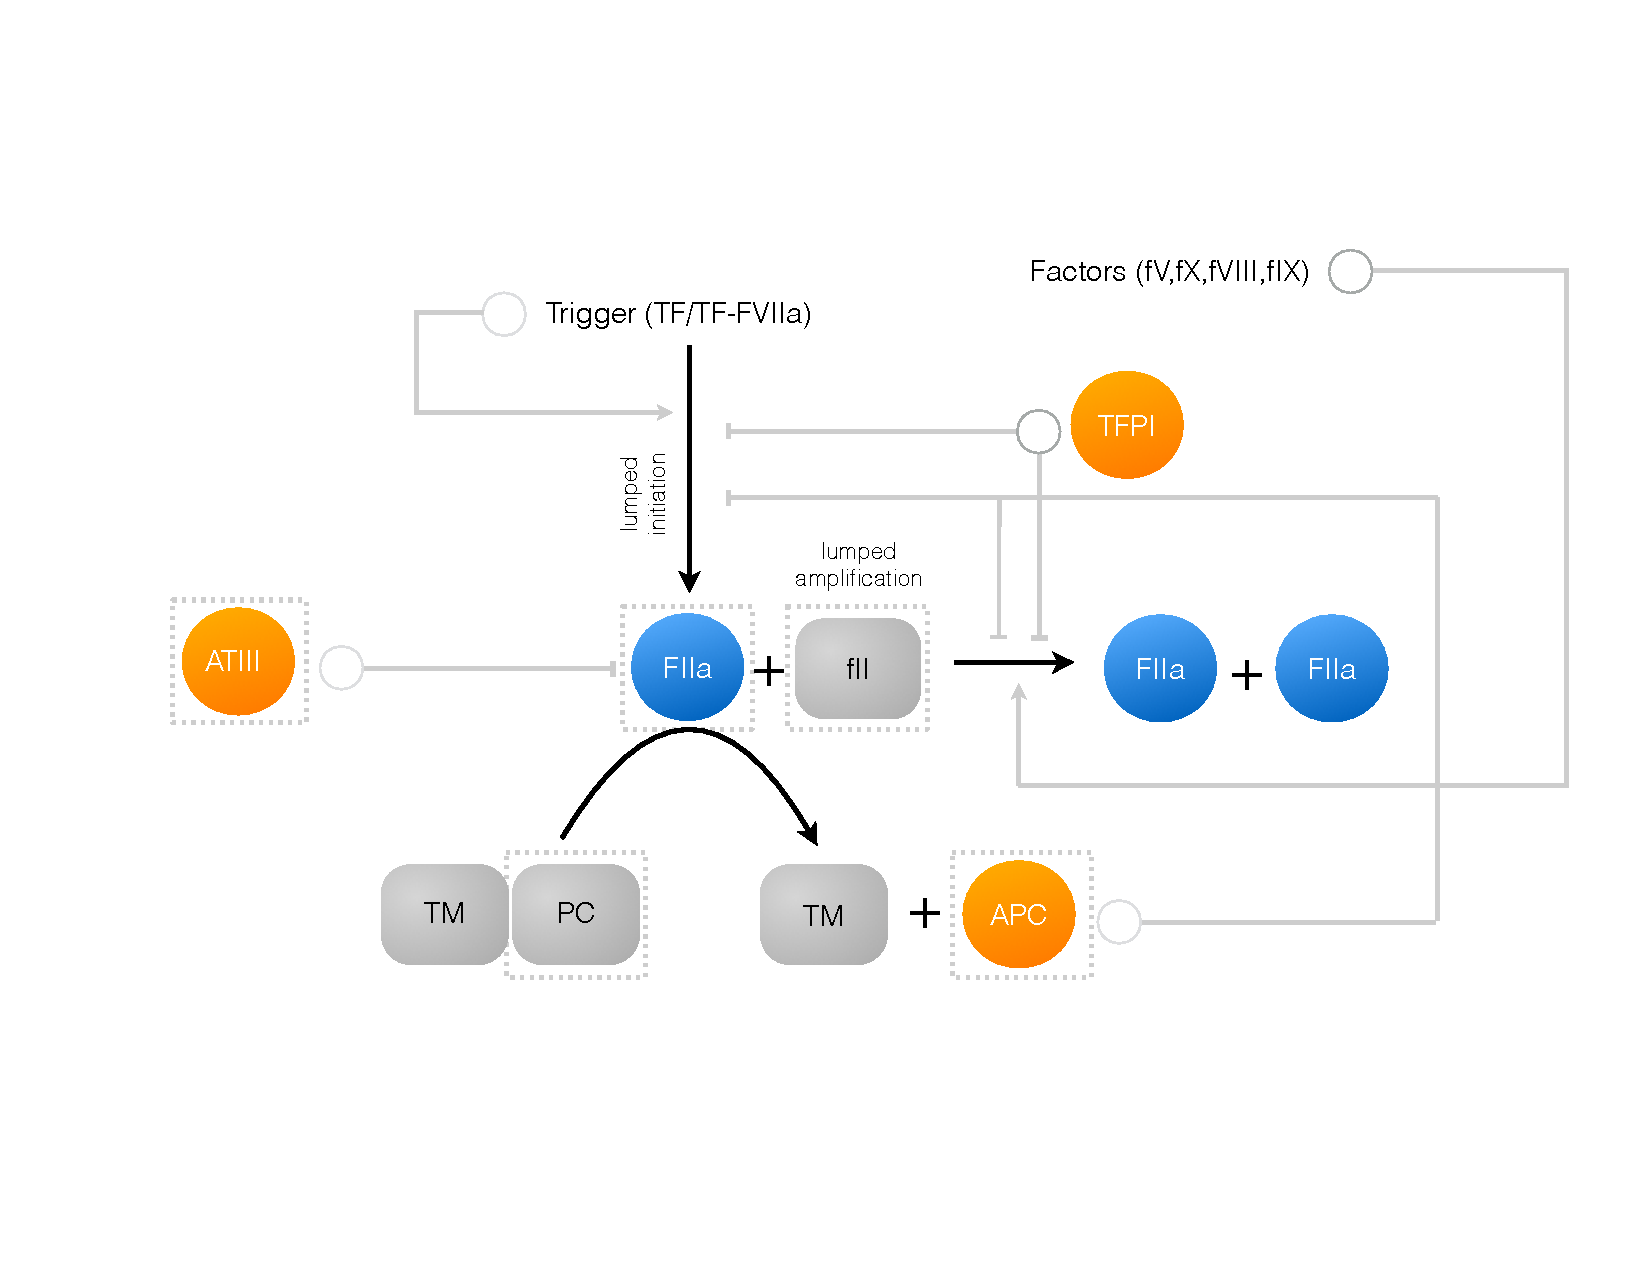
\includegraphics[width=1.0\textwidth]{./figs/Figure-1-Network.pdf}
\caption{Schematic of the connectivity of the reduced order coagulation model. A trigger compound, e.g., TF/FVIIa initiates thrombin production (FIIa) from prothrombin (fII).
Once activated, thrombin catalyzes its own activation (amplification step), as well as its own inhibition via the conversion of protein C to activated protein C (APC).
APC and tissue factor pathway inhibitor (TFPI) inhibit initiation and amplification, while antithrombin III (ATIII) directly inhibits thrombin. 
All inhibition steps and trigger-induced initiation were modeled using a rule-based approach. 
Likewise, the dependence of amplification on other coagulation factors was also modeled using a rule-based approach. 
The abundance of the highlighted species (in the dashed boxes) was governed by an ordinary differential equation. 
All other species were assumed to be constant.}\label{fig-network}
\end{figure}

\clearpage

\begin{figure}
\centering
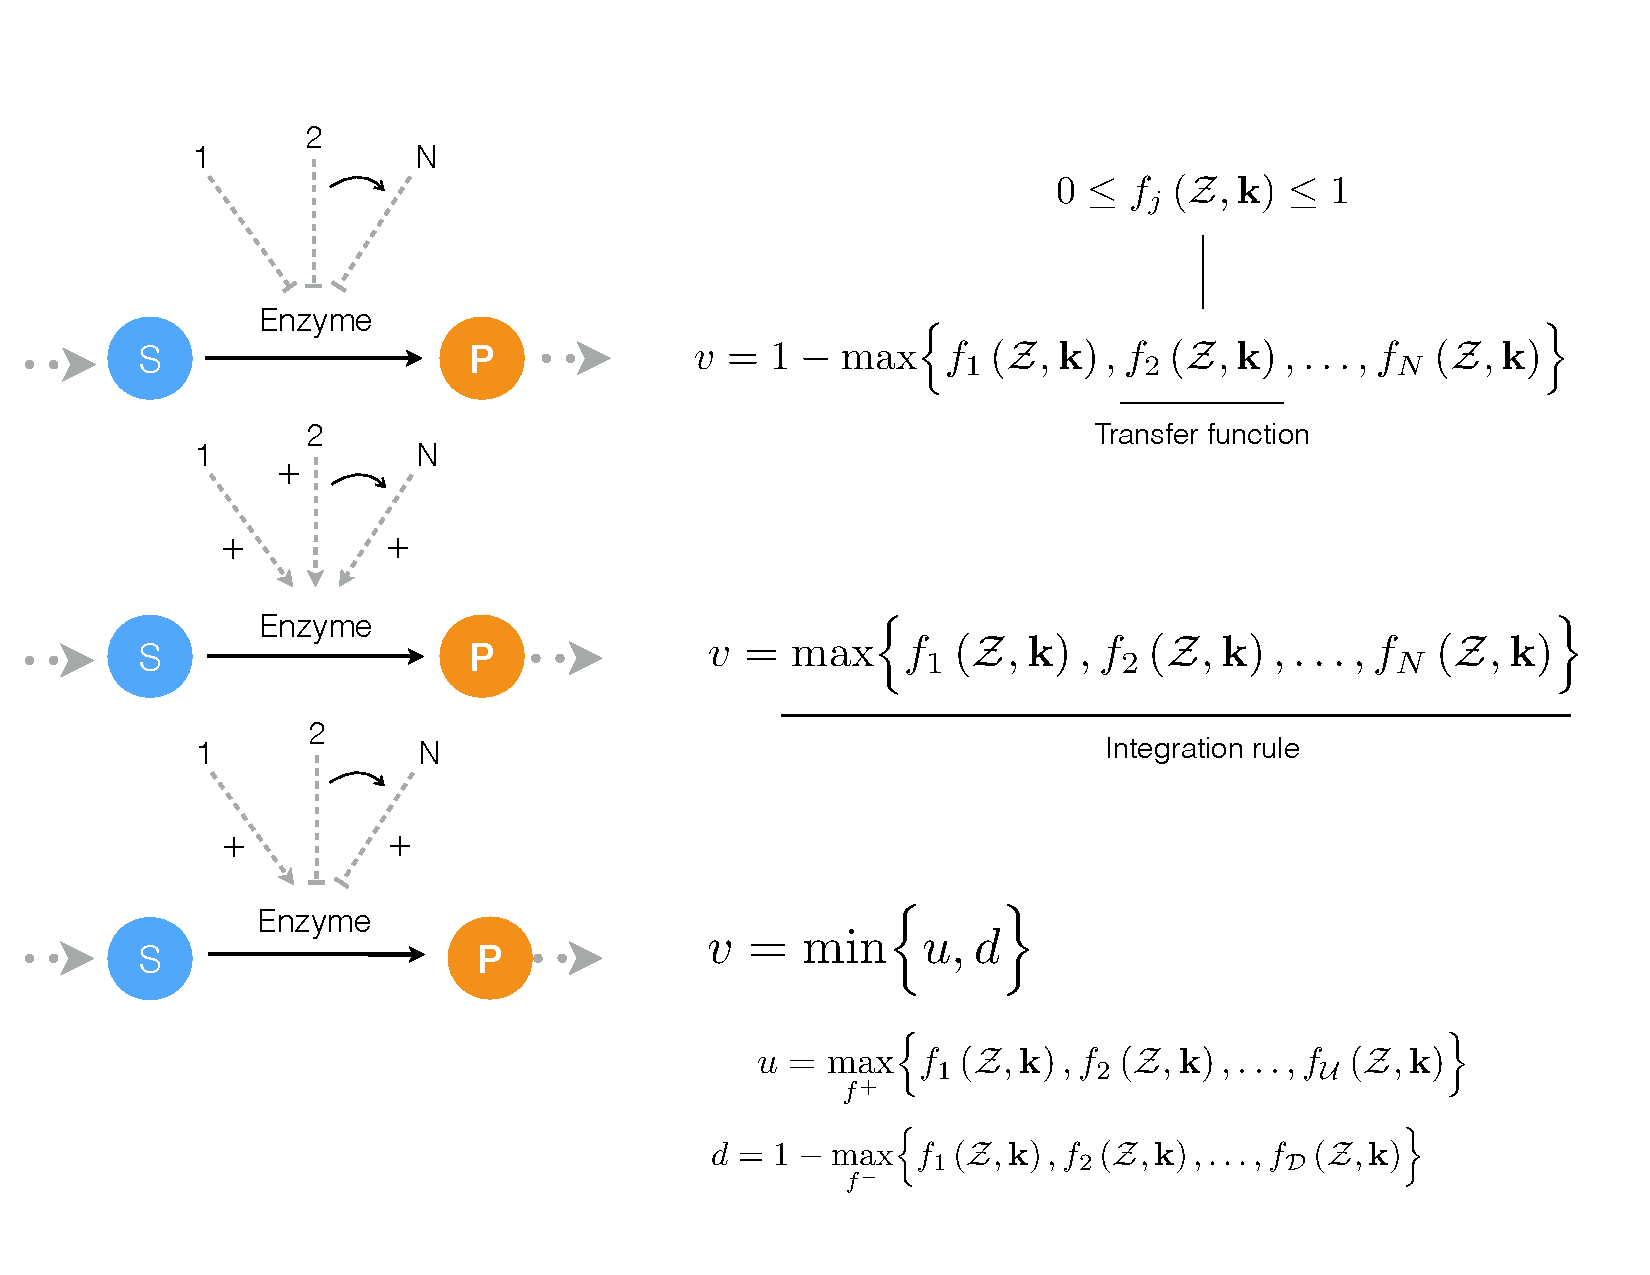
\includegraphics[width=1.0\textwidth]{./figs/Figure-2-ControlSchematic.pdf}
\caption{Schematic of rule-based effective control laws. 
Traditional enzyme kinetic expressions, e.g., Michaelis–Menten or multiple saturation kinetics are multiplied by an enzyme activity control variable $0 \leq v_{j} \leq 1 $. 
Control variables are functions of many possible regulatory factors encoded by arbitrary transfer functions of the form $0\leq f_{j}\left(\mathcal{Z}\right)\leq 1$.
At each simulation time step, the $v_{j}$ variables are calculated by evaluating integration rules such as the max or min of the set of transfer functions $f_{1},\hdots,f_{n}$ 
influencing the activity of enzyme $E_{j}$. }\label{fig-control-schematic}
\end{figure}

\clearpage

\begin{figure}
\centering
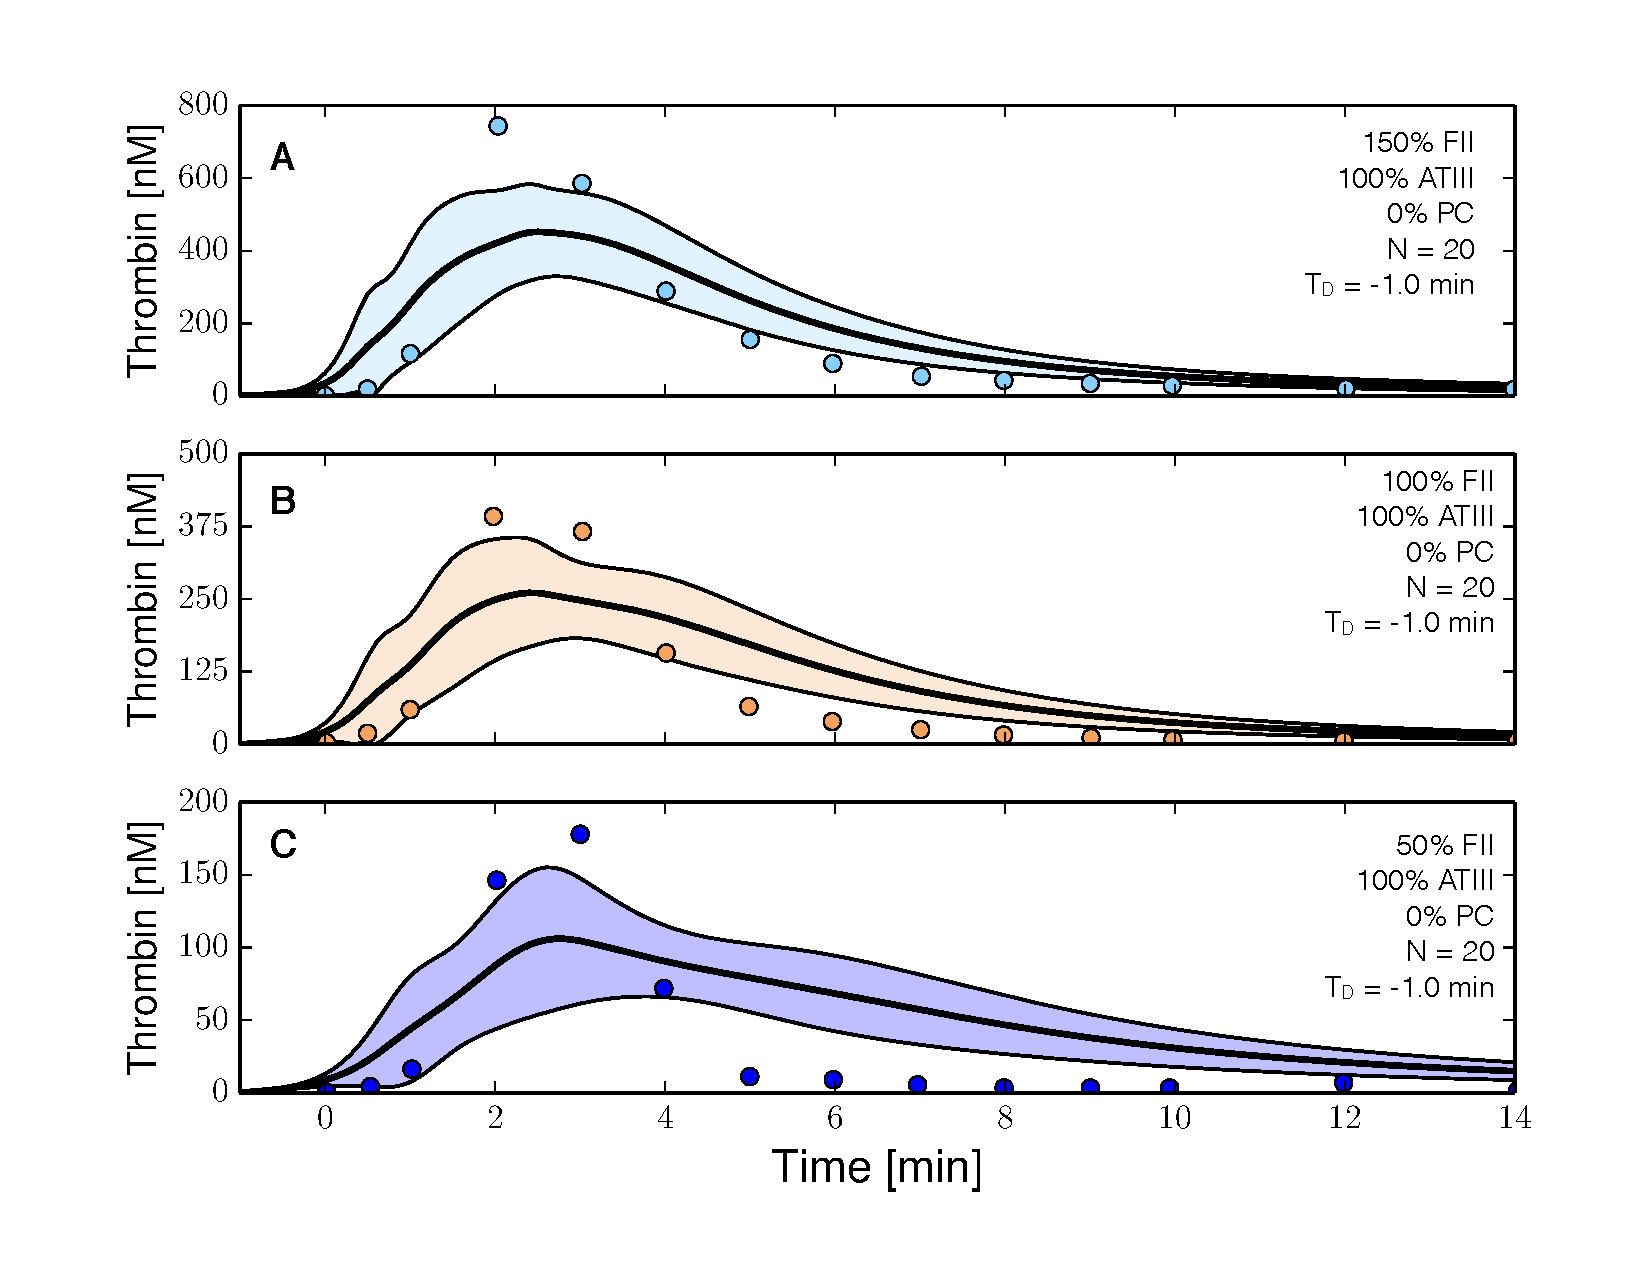
\includegraphics[width=1.0\textwidth]{./figs/Figure-3-DIFF_FII_NO_APC.pdf}
\caption{Reduced order coagulation model training simulations.
Reduced order coagulation model parameters were estimated using particle swarm optimization (PSO) with and without the protein C pathway as a function of prothrombin. 
Solid lines denote the simulated mean value of the thrombin profile for N = 20 independent particles, points denote experimental data. 
The shaded region denotes the 99\% confidence estimate of the mean simulated thrombin value (uncertainty in the model simulation).
(A,B,C) training results for 150\%, 100\% and 50\% of physiological prothrombin levels in the absence of the protein C pathway.
Thrombin generation was initiated using 5 pmol/L FVIIa-TF in the presence of 200 $\mu$mol/L of phospholipid vesicles (PCPS). 
All factors and control proteins were at their physiological concentration unless others denoted. 
The experimental training data was reproduced from the study of Butenas \textit{et al.} \citep{Butenas:1999aa}.}\label{fig-diff_fII_NO_APC}
\end{figure}

\clearpage

\begin{figure}
\centering
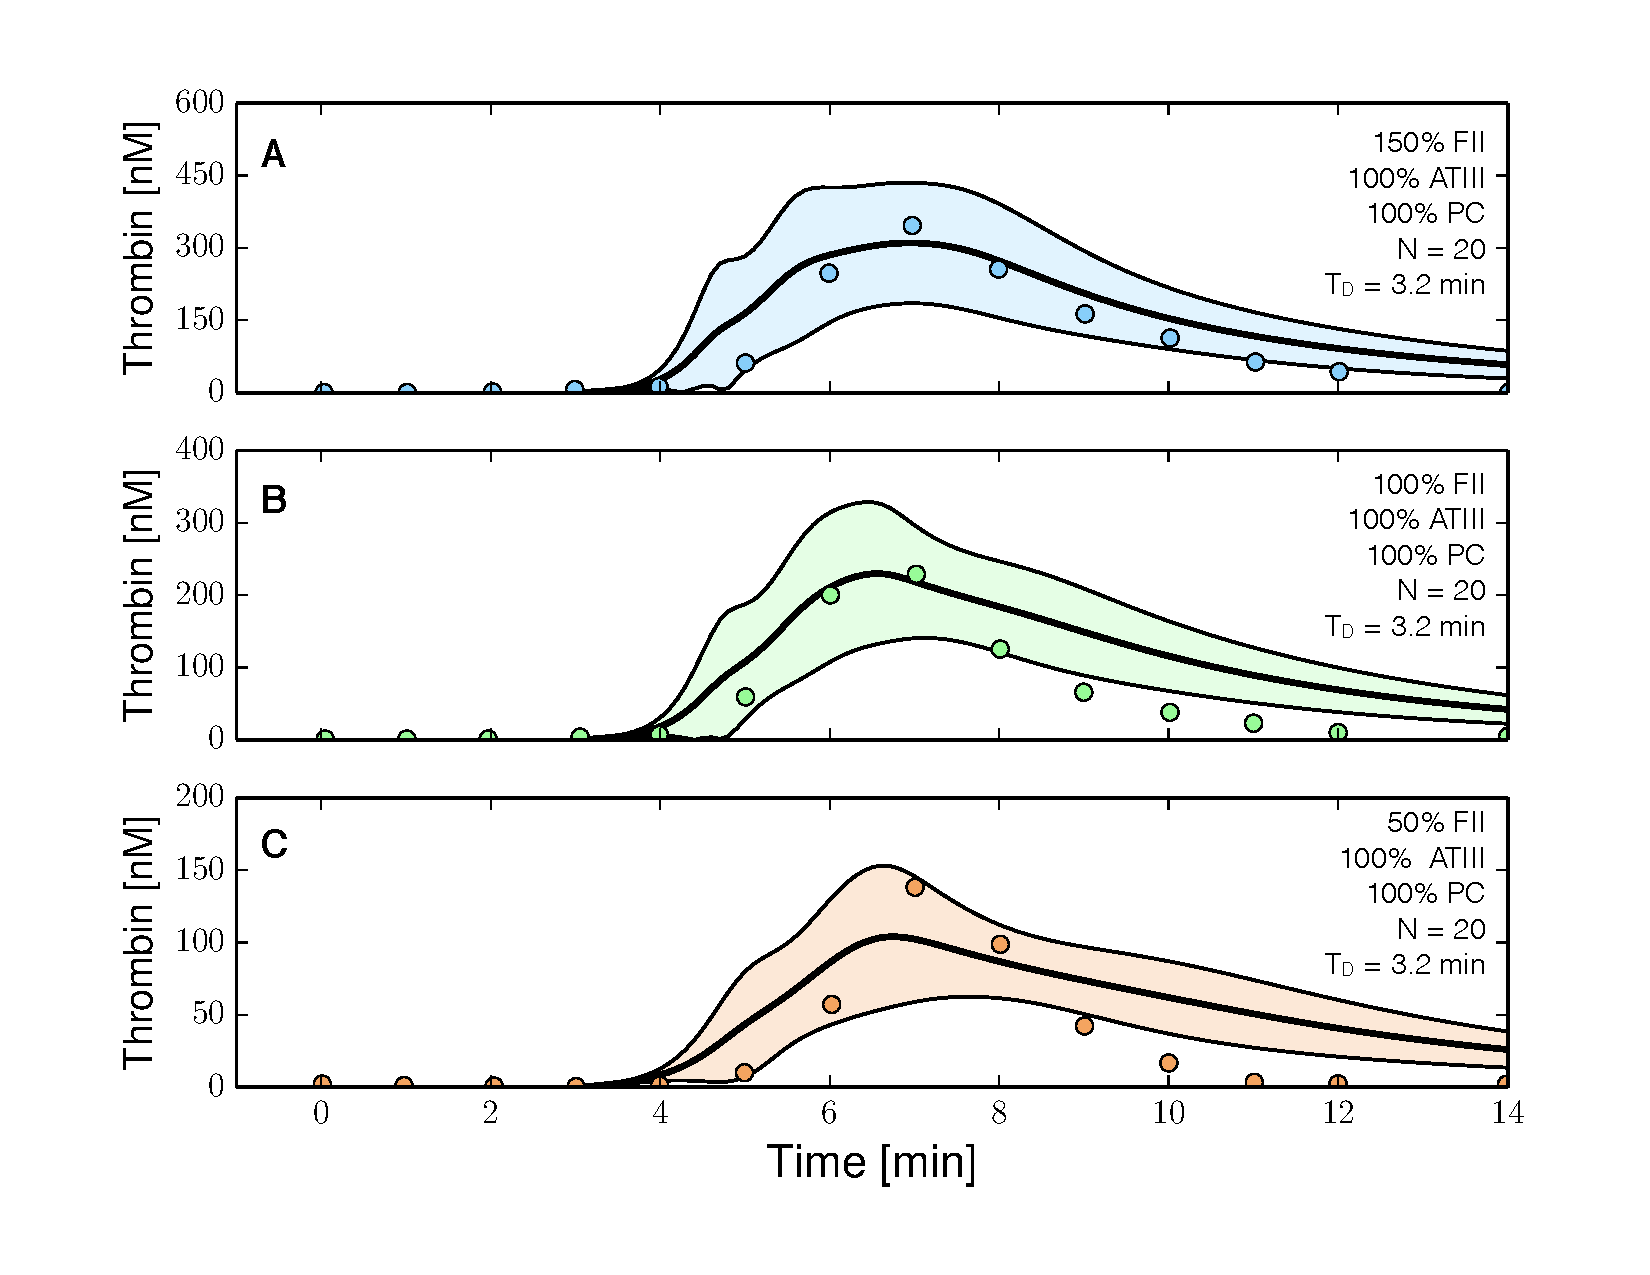
\includegraphics[width=1.0\textwidth]{./figs/Figure-4-DIFF_FII_APC.pdf}
\caption{Reduced order coagulation model training simulations.
Reduced order coagulation model parameters were estimated using particle swarm optimization (PSO) with and without the protein C pathway as a function of prothrombin. 
Solid lines denote the simulated mean value of the thrombin profile for N = 20 independent particles, points denote experimental data.
The shaded region denotes the 99\% confidence estimate of the mean simulated thrombin value (uncertainty in the model simulation).
(A,B,C) training results for 150\%, 100\% and 50\% of physiological prothrombin levels in the presence of the protein C pathway. 
Only APC pathway parameters were allowed to vary in the simulations on the right.
Thrombin generation was initiated using 5 pmol/L FVIIa-TF in the presence of 200 $\mu$mol/L of phospholipid vesicles (PCPS). 
All factors and control proteins were at their physiological concentration unless others denoted.
The experimental training data was reproduced from the study of Butenas \textit{et al.} \citep{Butenas:1999aa}.}\label{fig-diff_fII_APC}
\end{figure}

\clearpage

\begin{figure}
\centering
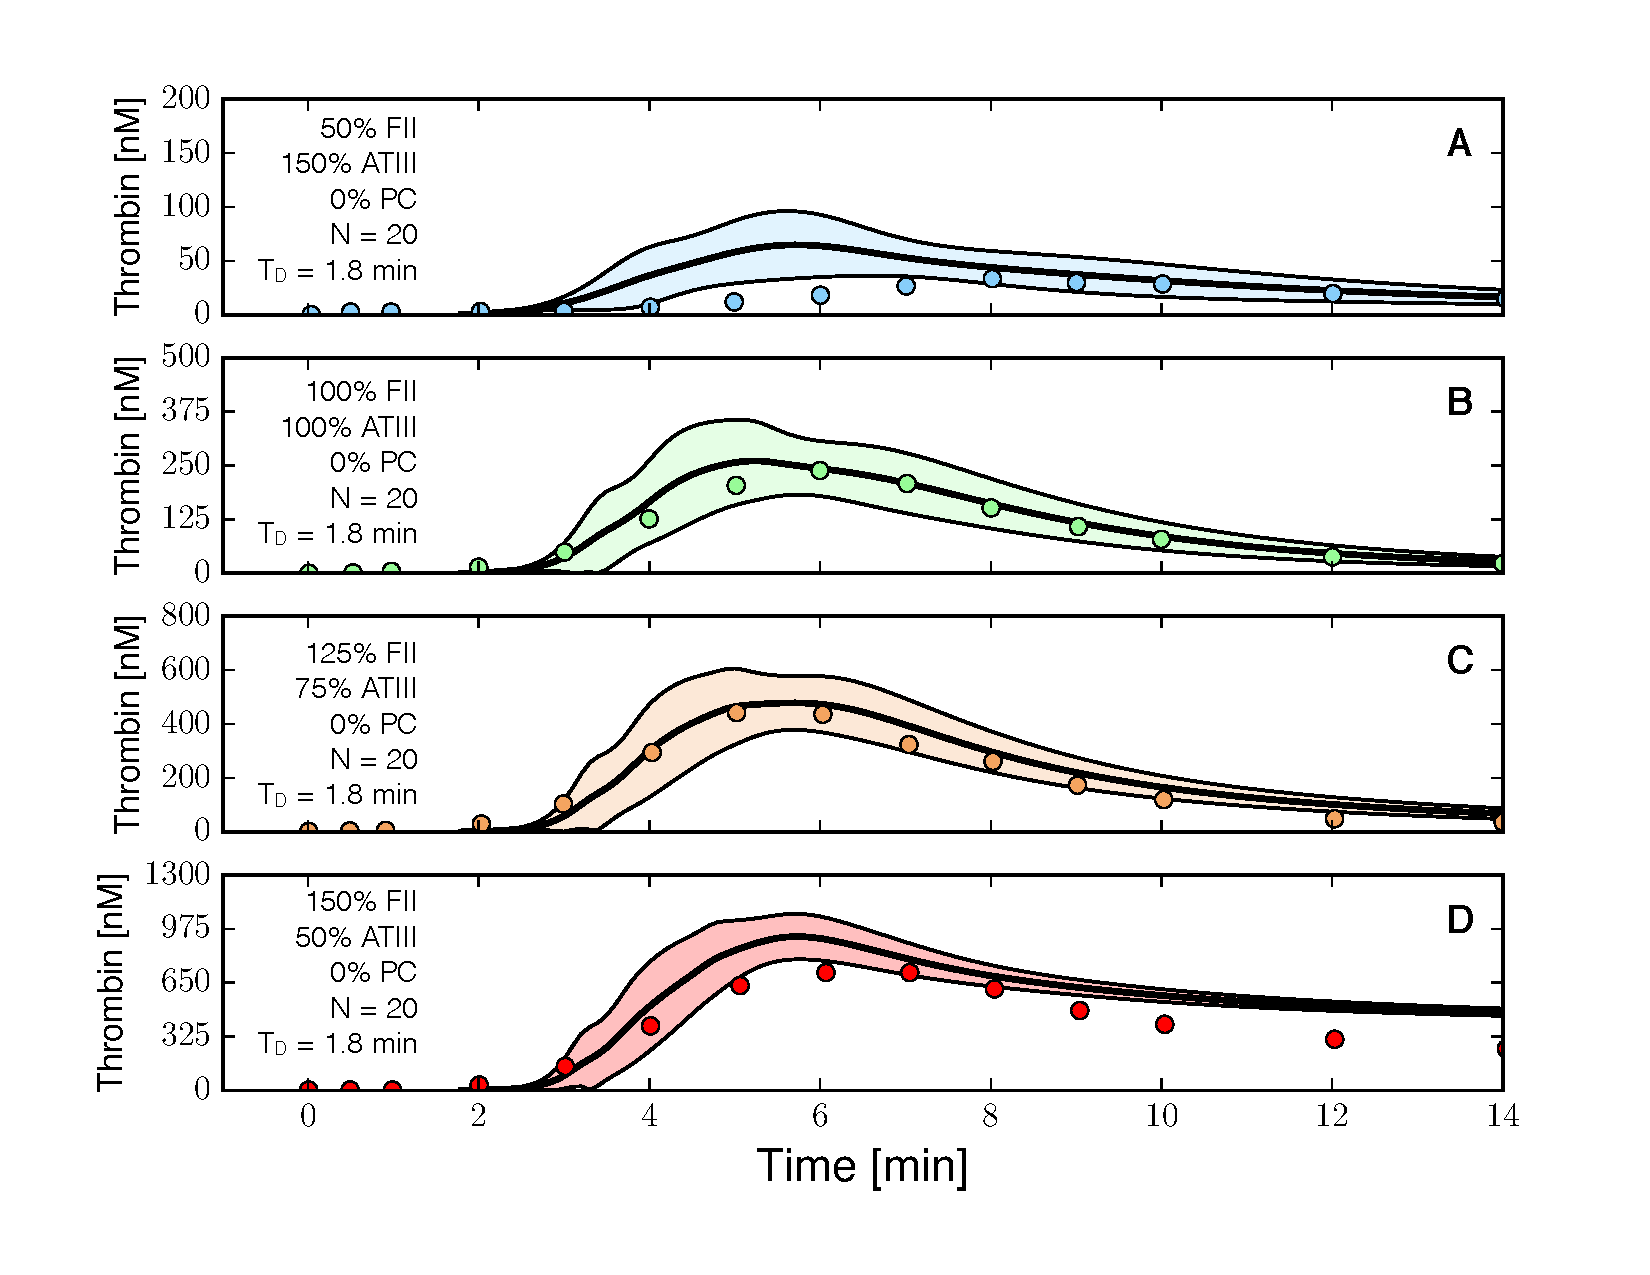
\includegraphics[width=1.0\textwidth]{./figs/Figure-5-FII_ATIII.pdf}
\caption{Reduced order coagulation model predictions versus experimental data for normal coagulation. 
The reduced order coagulation model parameter estimates were tested against data not used during model training.
Simulations of different levels of prothrombin and ATIII were compared with experimental data in the absence of the protein C pathway. 
Solid lines denote the simulated mean value of the thrombin profile for N = 20 independent particles, points denote experimental data.
The shaded region denotes the 99\% confidence estimate of the mean simulated thrombin value (uncertainty in the model simulation). 
(A,B,C,D) prediction results for (FII,ATIII): (50\%,150\%), (100\%, 100\%), (125\%, 75\%) and (150\%, 50\%) of physiological prothrombin and ATIII levels in the absence of the protein C pathway. 
Thrombin generation was initiated using 5 pmol/L FVIIa-TF in the presence of 200 $\mu$mol/L of phospholipid vesicles (PCPS). 
All factors and control proteins were at their physiological concentration unless others denoted.
The experimental validation data was reproduced from the study of Butenas \textit{et al.} \citep{Butenas:1999aa}}\label{fig-fII_ATIII}
\end{figure}

\clearpage

\begin{figure}
\centering
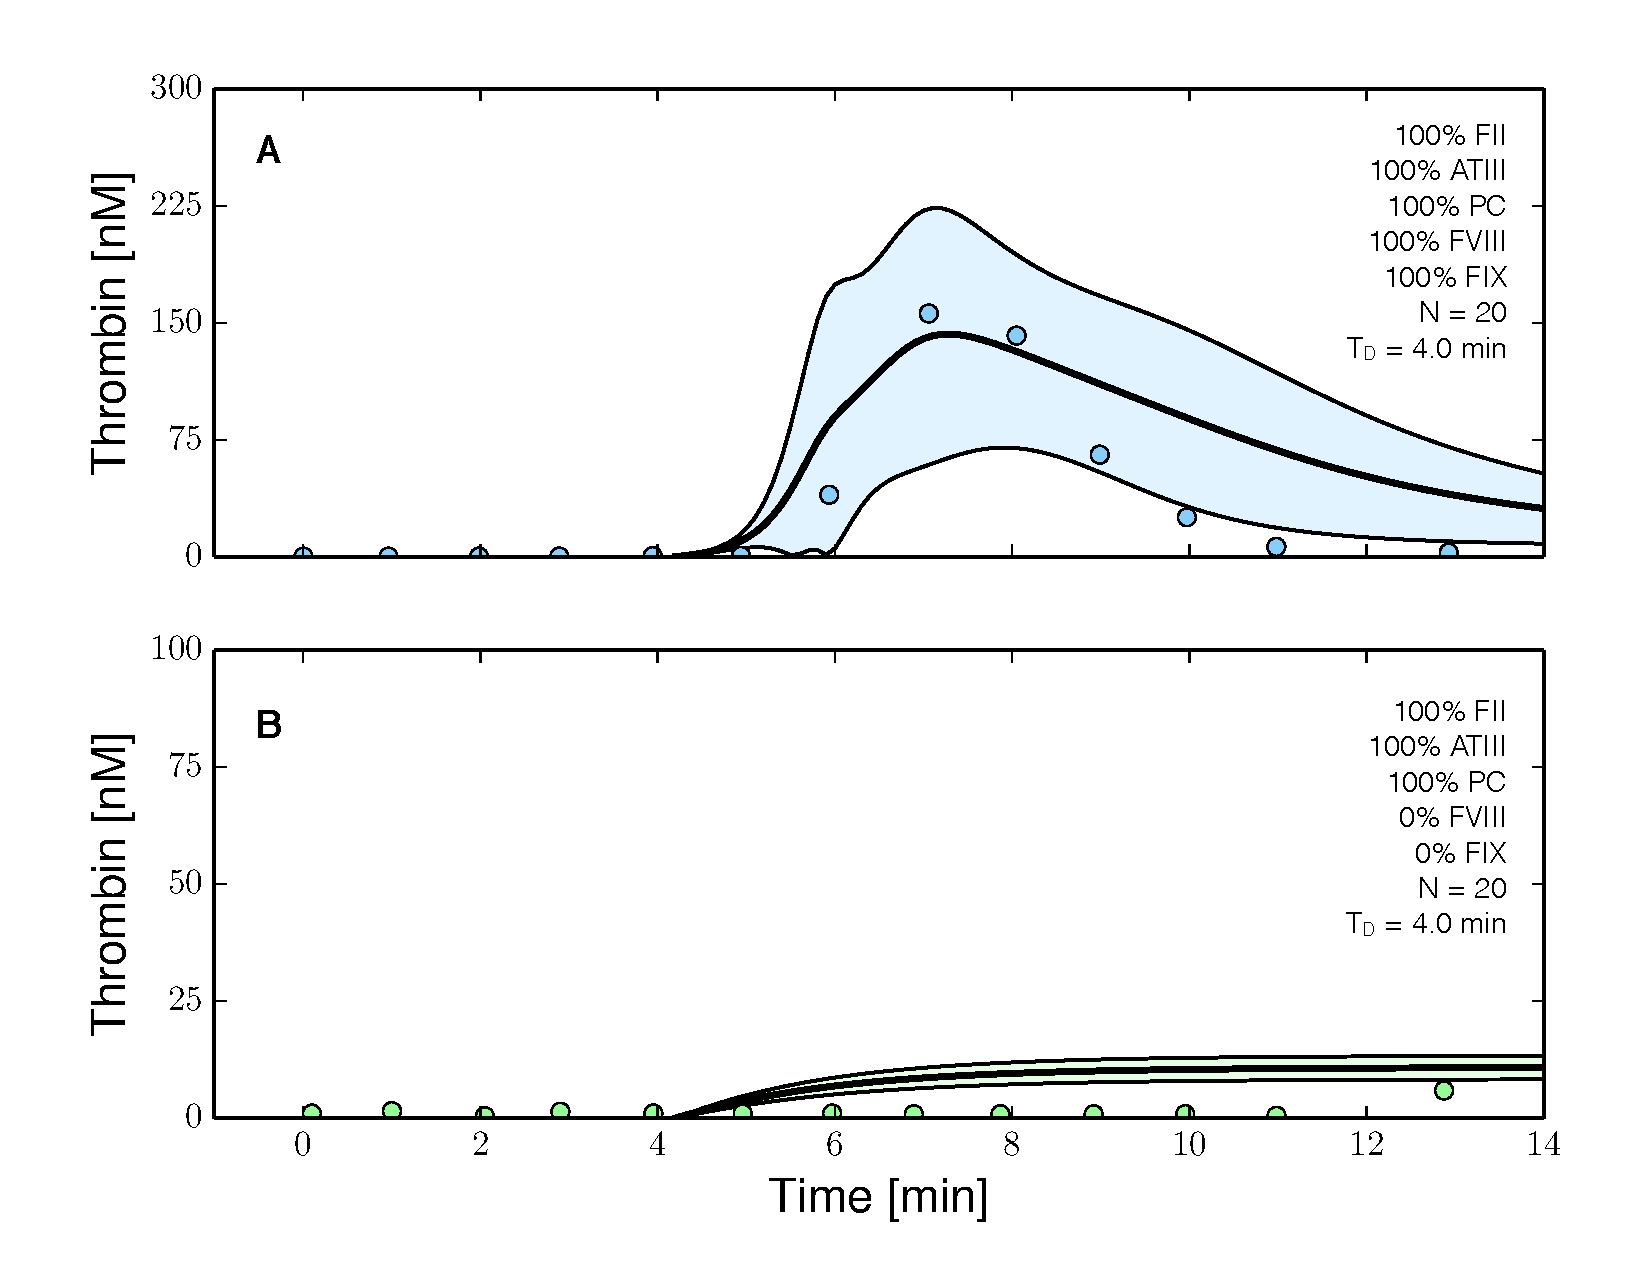
\includegraphics[width=1.0\textwidth]{./figs/Figure-6-Hemophilia.pdf}
\caption{Reduced order coagulation model predictions versus experimental data with and without FVIII and FIX.
The reduced order coagulation model parameter estimates were tested against data not used during model training. 
Simulations of normal thrombin formation with ATIII and the protein C pathway were compared with thrombin formation in the absence of fVIII and fIX.
Solid lines denote the simulated mean value of the thrombin profile for N = 20 independent particles, points denote experimental data.
The shaded region denotes the 99\% confidence estimate of the mean simulated thrombin value (uncertainty in the model simulation). 
(A,B) prediction results for normal thrombin generation and thrombin generation in hemophilia. 
All factors and control proteins were at their physiological concentration unless others noted.
The experimental validation data was reproduced from the study of Allen \textit{et al.} \citep{ALLEN2006}.}\label{fig-hemophilia}
\end{figure}

\clearpage

\begin{figure}
\centering
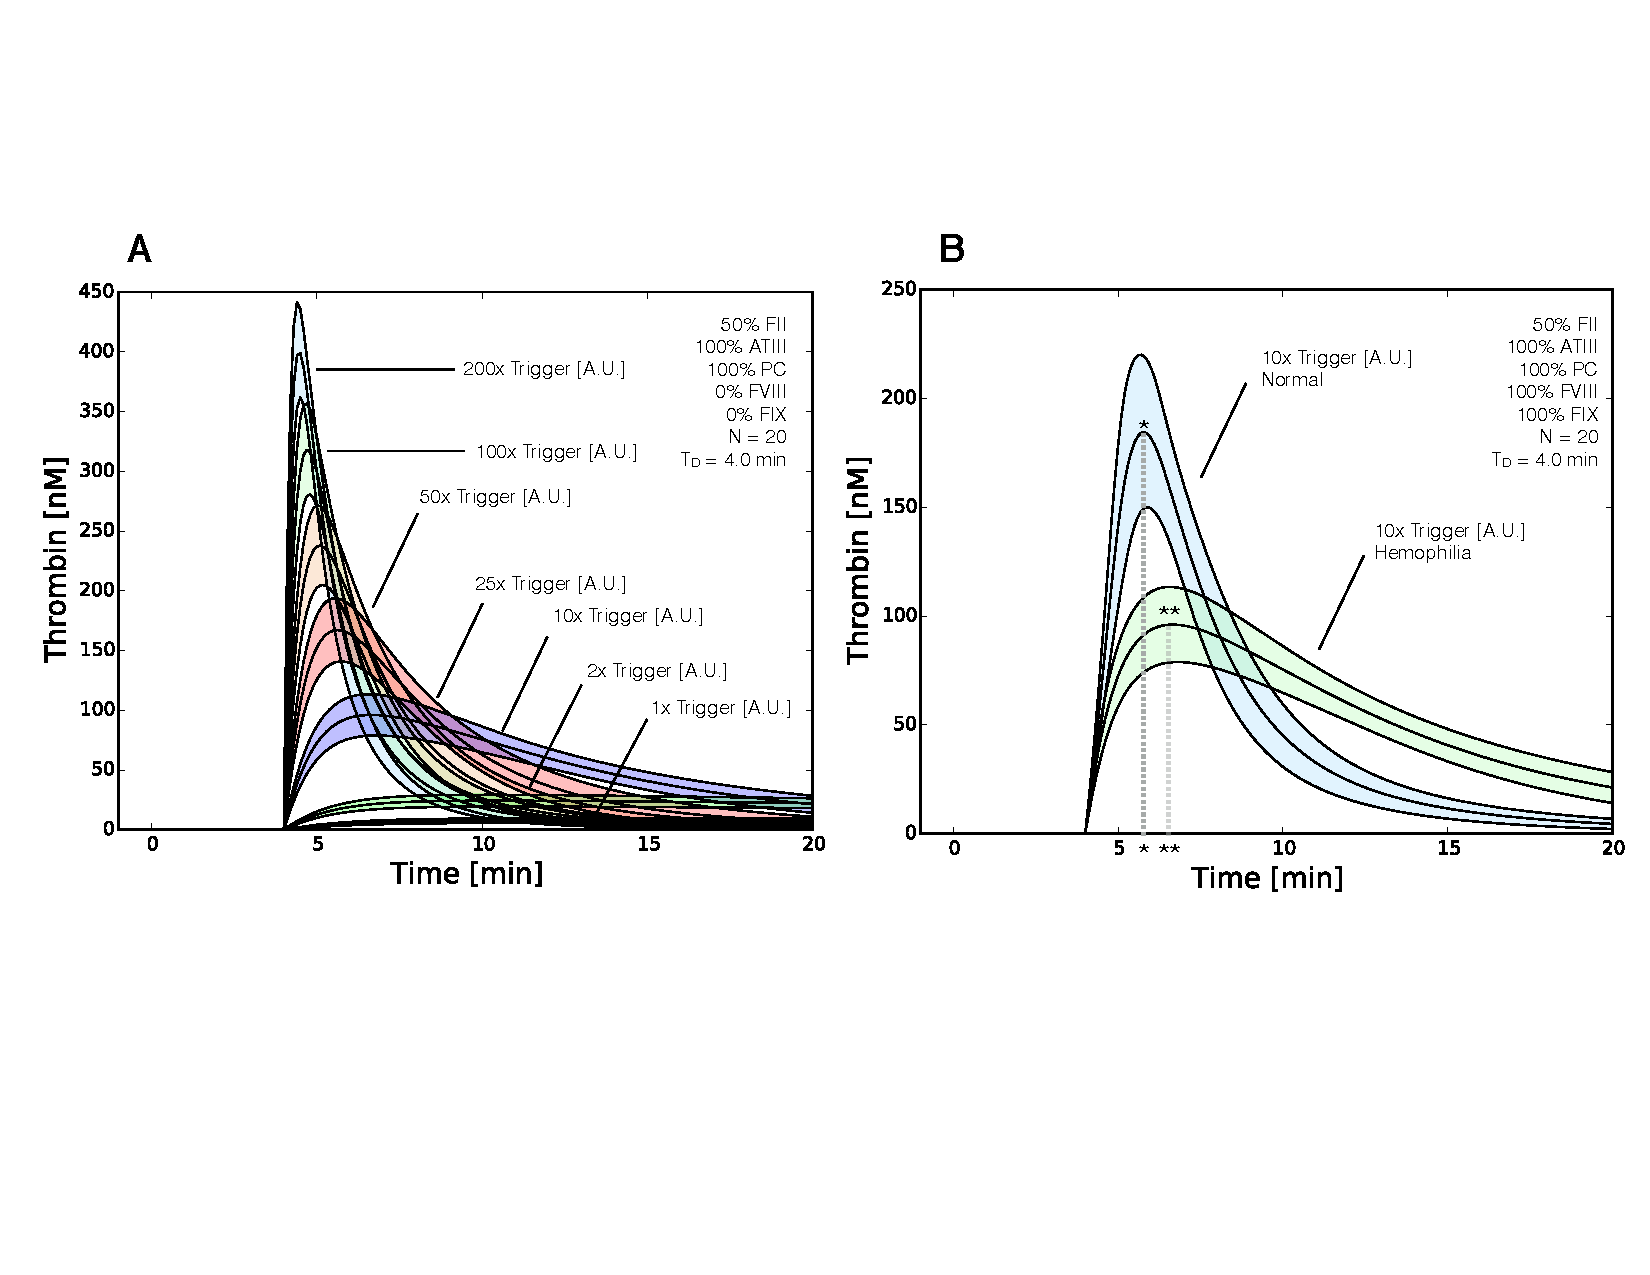
\includegraphics[width=1.0\textwidth]{./figs/Figure-7-rFVIIa-Trigger.pdf}
\caption{Reduced order coagulation model predictions of rFVIIa administration. 
A: Simulations of thrombin formation in the presence of ATIII and the protein C pathway were conducted for a range of trigger values (1x - 200x nominal) in the absence of fVIII and fIX.
B: Comparison of thrombin generation for normal versus hemophilia for 10x nominal trigger.
Solid lines denote the simulated mean value of the thrombin profile for N = 20 independent particles. 
The peak thrombin time for normal coagulation ($t^{*}$) is less than rFVIIa induced coagulation in hemophilia ($t^{**}$), while the peak thrombin value was greater in normal coagulation.
The shaded region denotes the 99\% confidence estimate of the mean thrombin value (uncertainty in the model simulation). 
All factors and control proteins were at their physiological concentration unless others noted.}\label{fig-rFVII}
\end{figure}

\clearpage

\begin{figure}
\centering
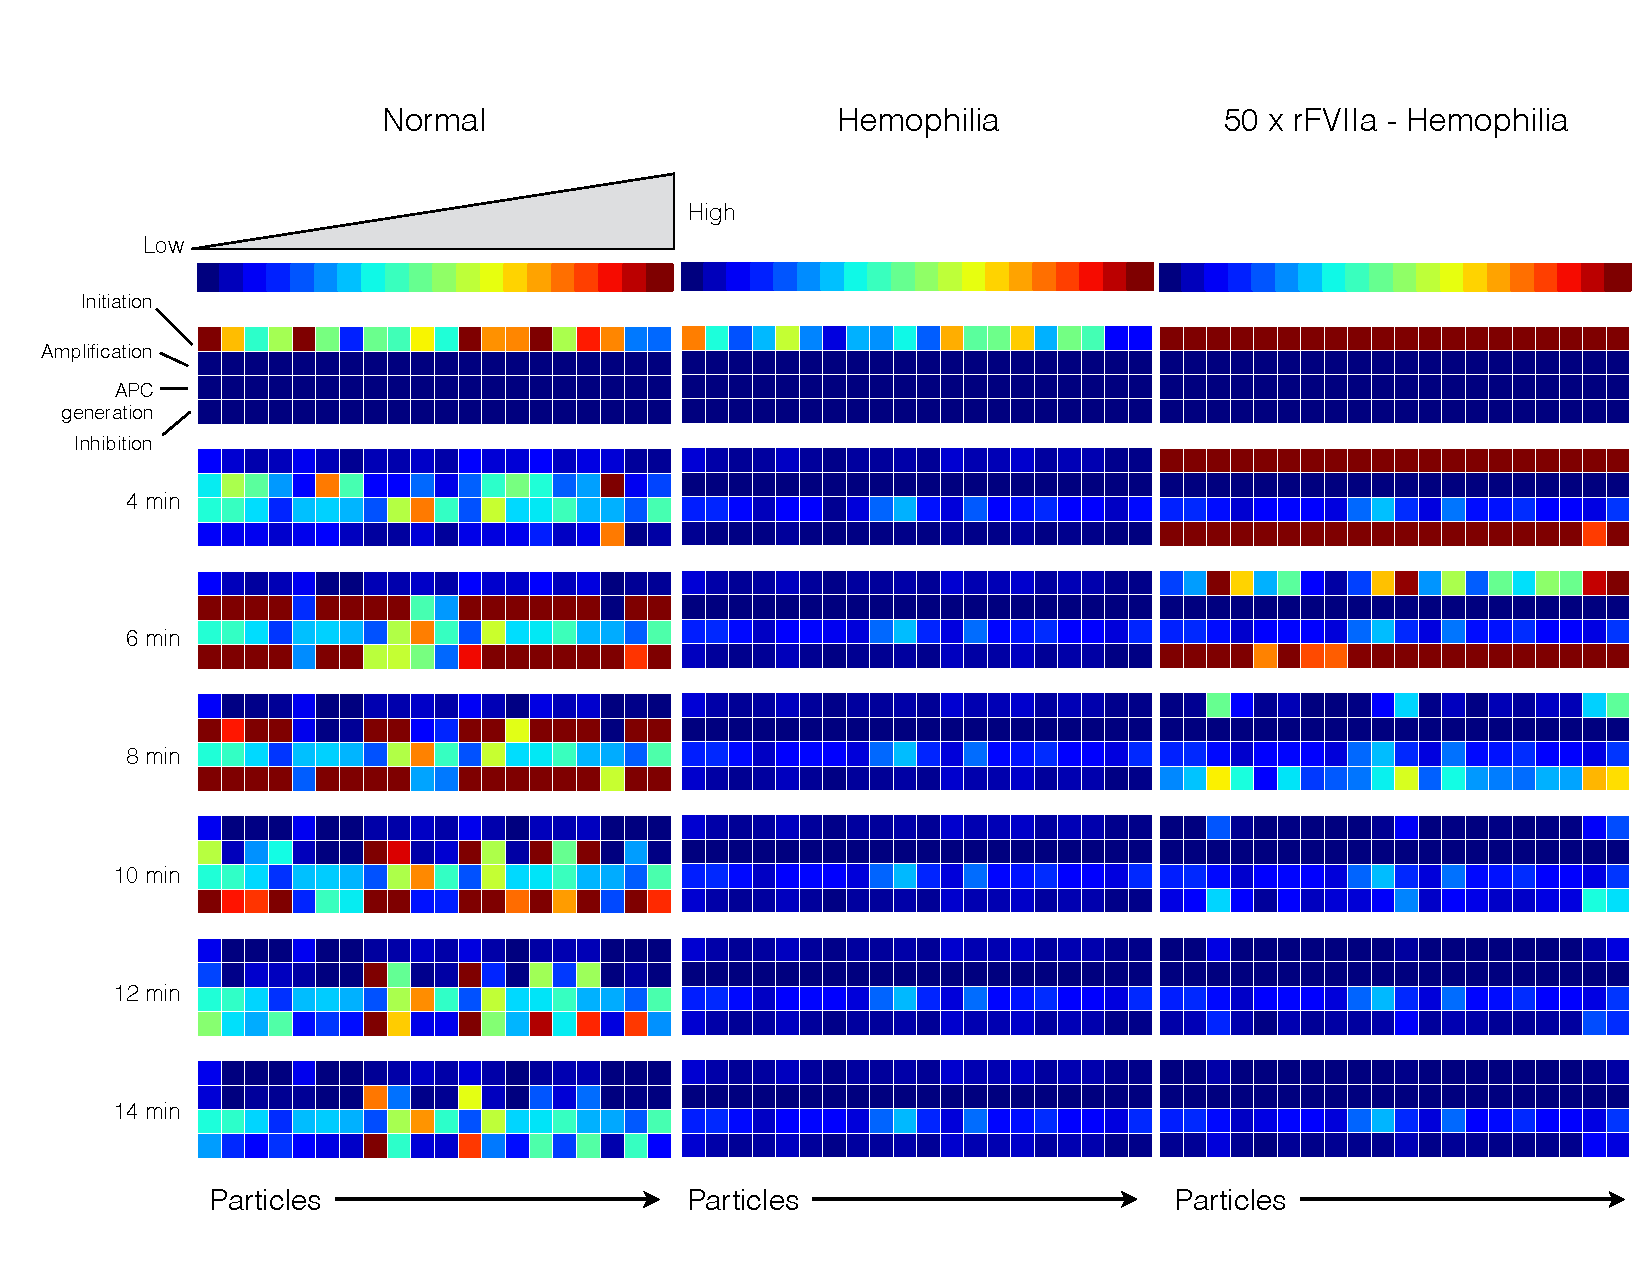
\includegraphics[width=1.0\textwidth]{./figs/Figure-8-Flux-rFVIIa-Trigger.pdf}
\caption{Reaction flux distribution as a function of time for thrombin generation under normal (left), hemophilia (center) and rFVIIa treated hemophilia (right).
Reaction flux was calculated for each particle at $T = 0,4,6,8,10,12,14$ min after the initiation of coagulation. 
Reaction fluxes were calculated for each particle in the parameter ensemble (N = 20).
Blue colors denote low flux values while red colors denote high flux values.}\label{fig-flux-analysis}
\end{figure}

\clearpage

\begin{figure}
\centering
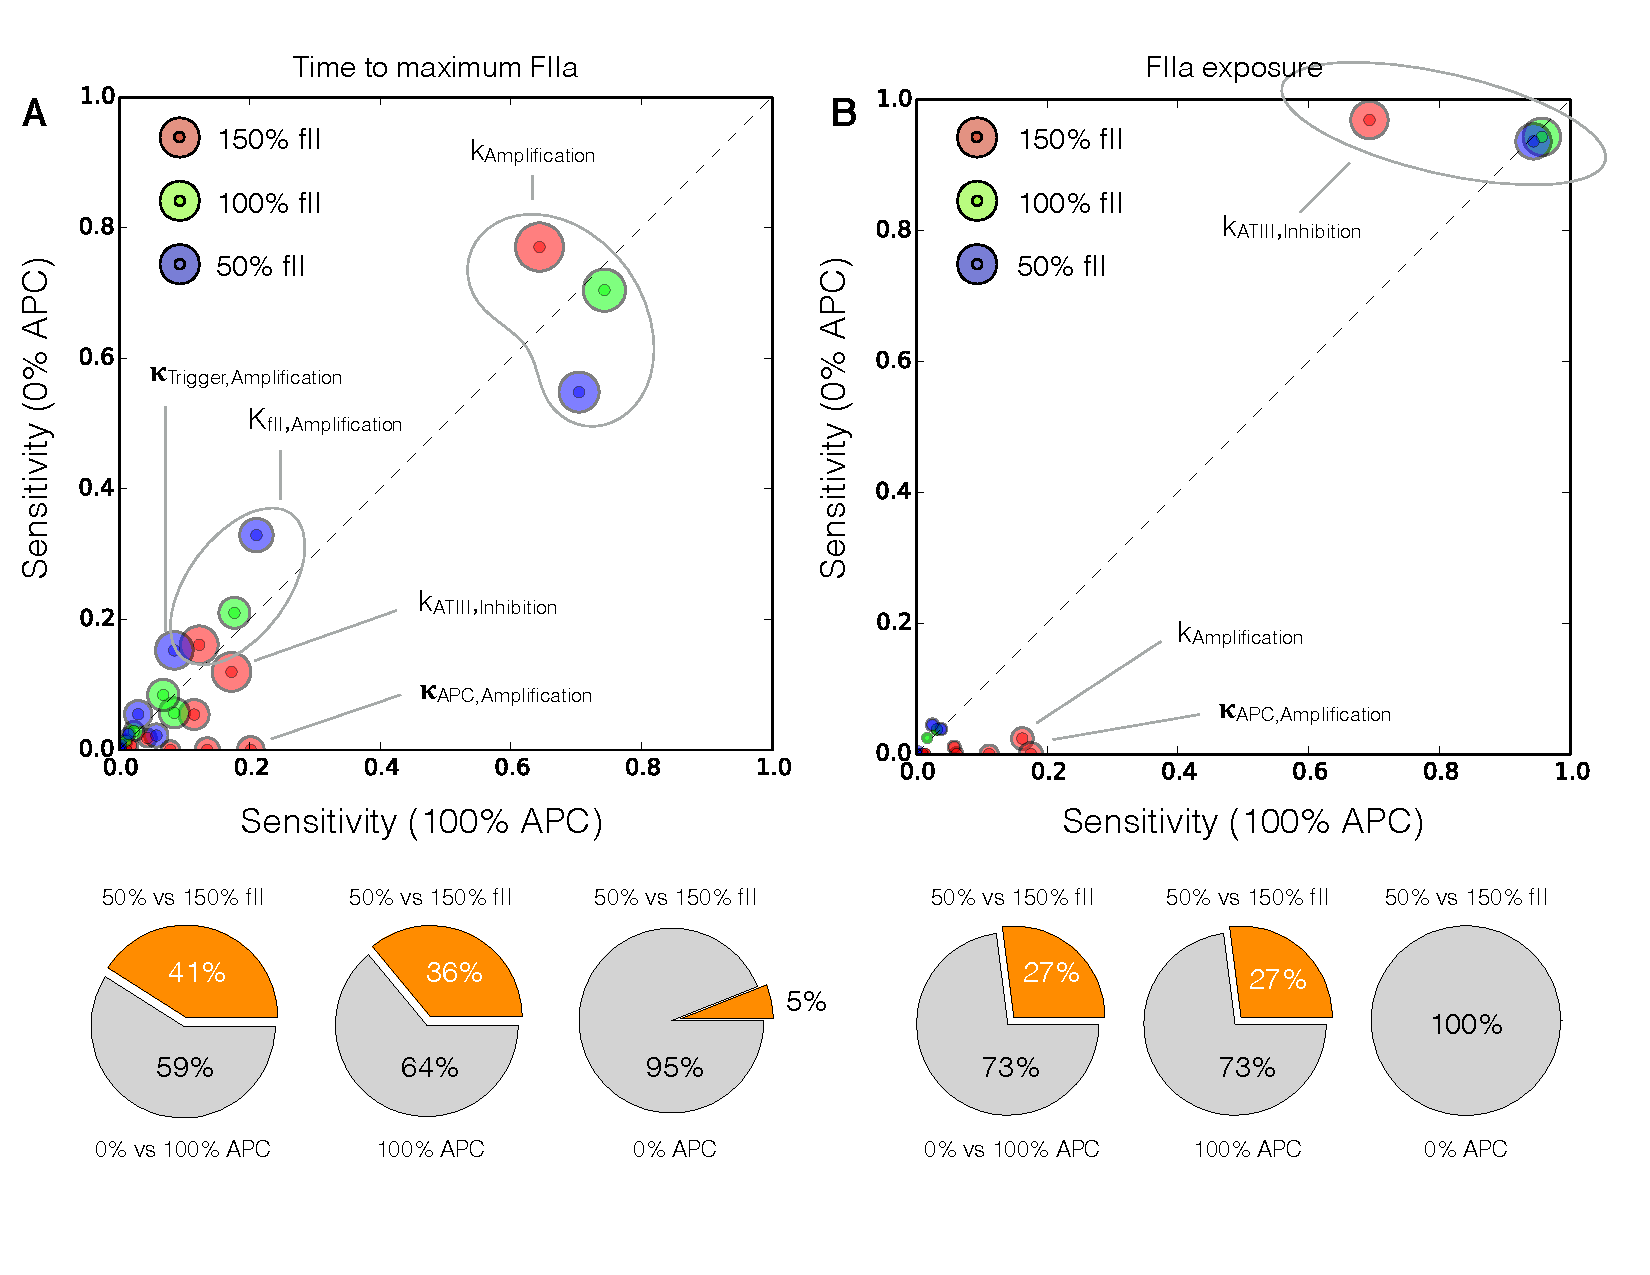
\includegraphics[width=1.0\textwidth]{./figs/Figure-9-Sensitivity.pdf}
\caption{Global sensitivity analysis of the reduced order coagulation model with respect to the model parameters.
A: Sensitivity analysis of the thrombin peak time for different prothrombin levels (150\%,100\% and 50\% of the physiological value) as a function of activated protein C. 
B: Sensitivity analysis of the thrombin exposure for different prothrombin levels (150\%,100\% and 50\% of the physiological value) as a function of activated protein C. 
Points denote the mean total sensitivity value, while the area around each point denotes the uncertainty in the sensitivity value. 
The gray dashed line denotes the 45$^{\circ}$ degree diagonal, if sensitivity values are equal for different conditions they will lie on the diagonal.  
Sensitivity values significantly above or below the diagonal indicate differentially important model parameters. 
The radius of the shaded region around each total sensitivity value was the maximum uncertainty in that value estimated by the Sobol method. 
}\label{fig-sensitivity}
\end{figure}

\clearpage

% Supplemental figures -
% Set the S- 
\renewcommand\thefigure{S\arabic{figure}}
\renewcommand\thetable{T\arabic{table}}
\renewcommand\thepage{S-\arabic{page}}
\renewcommand\theequation{S\arabic{equation}}

% Reset the counters -
\setcounter{equation}{0}
\setcounter{table}{0}
\setcounter{figure}{0}
\setcounter{page}{1}

\end{document}

